%note pour les g\'en\'erations suivantes : ceci est la version 2012 de l'infoBR par les infoBRmen 2011 : Arcos, gerard, Thunder ainsi que Chantal pour les couv. 


%La structure g\'en\'erale du document date de 2009 au moins, nous n'y avons pas touch\'e. Elle est tr\`es pratique pour ne pas avoir un .tex \'enorme dans lequel on ne retrouve rien. Si suite \`a une erreur quelconque dans un des fichiers (typiquement : une balise de fin de liste oubli\'ee), la compilation m\`ene \`a une erreur et ne termine pas, corriger l'erreur dans le fichier concern\'e et relancer la compilation. Le fichier peut alors refuser de compiler (affiche une erreur \`a la ligne \begin{document}. Balancer le fichier .aux \`a la poubelle r\`egle le probl\`eme.


%Le gros changement dans cette version est la baisse drastique du nombre de pages, qui passent de 42 pages pour la version 2011 \`a 28 pages pour cette version 2012. La principale raison de ce changement est le co\^ut d'impression. On ne peut pas demander \`a la promo de payer des milliers d'euros pour des pages compl\`etement inutiles ou qui ne sont lues que par 3 personnes. L'autre est qu'un document aussi long d\'ecourageait toute lecture. Nous avons donc vir\'e pas mal de trucs, en essayant au maximum de mettre les info concern\'ees sur le wikiBR et d'inciter les gens \`a y aller. 


% il peut rester des restes de cet \'elagage, nous avons comment\'e certains appels \`a des fichiers  ou morceaux de texte plut�t que de tout effacer.

%Note du BR 2012: nous avons réintroduit la section sur Frankiz, pour essayer de maximiser le nombre de gens qui sont au courant des diverses possibilités du site.
%La section est longue, mais le nombre de pages devant être multiple de 4 elle ne change pas le nombre de pages total (28).
%Nous avons aussi tout passé en niveaux de gris pour baisser encore les coûts d'impression

% -------------------- Header --------------------
\documentclass[12pt, a4paper, twoside]{article}
\usepackage{preambuleInfoBR}

\title{InfoBR 2012}
\author{Binet R\'eseau 2k12}
\date{ }
\usepackage{garamond}



\begin{document}

\garamond
\setlength{\parskip}{0pt plus 2ex}
 



% ------------------------------ Exergue ------------------------------
% on peut l'enlever, selon le nombre de pages \`a atteindre

%\thispagestyle{empty}
\vspace*{\stretch{1}}

\begin{center}
\begin{Huge}
InfoBR 2k8
\end{Huge}
\end{center}

\vspace*{\stretch{1}}

\begin{flushright}
\begin{large} 
 {\fontfamily{pzc} \selectfont
\`A mes illustres prédécesseurs:\\
\smallskip
mYk, bernardofpc, questor, eracil \\ }
\end{large}
\vspace{1cm}
{Palaiseau, le \today \\
\medskip
 j-philippe, InfoBR-man 2k7  }
\end{flushright} 

%\vspace*{\stretch{2}}

\newpage

\thispagestyle{plain}


\hrulefill \, \begin{Large}Notes personnelles\end{Large} \hrulefill

 
%\newpage

% -------------------- Le mot du prez: ----- 'motPrez.tex' --------------------
%\thispagestyle{empty}
%\setcounter{page}{1}
%\markright{Mot du prez}


%\input{motPrez2010}


%note : cette page a \'et\'e supprim\'ee dans la version 2012 et le mot du prez a fusionn\'e avec la partie avertissement (cf la section suivante).

\newpage



% -------------------- Le mot du redacteur: ----- 'avertissement.tex' --------------------

\markright{Introduction}

\begin{center}
\Large{Le mot du prez}
\end{center}
 Bonjour \`a tous !!


\newpage

\renewcommand{\contentsname}{Sommaire}
\bghdr{images/fond-infobr} \markright{Table des mati\`eres}

\tableofcontents

\newpage

% -------------------- Premiers pas : --------------------
\section{Premiers pas\ldots} \markright{Pour bien commencer}

% -------------------- Les differentes configs --------------------

\markright{Configuration sous Windows} \label{windows}
\bghdr{images/fond-win}

%\begin{center}
%
\includegraphics{images/logo_Windows}
%\end{center}


\subsection{Configuration sous Microsoft Windows}

%Cette section décrit comment configurer un ordinateur tournant sous Windows XP, Windows Vista, Windows 7 ou Windows 8. Si tu possèdes une autre version de Windows,
%nous t'invitons à  regarder directement la section sur les licences MSDNAA en page \pageref{msdnaa}\dots ou alors à  te débrouiller ! ;-)
%
%\subsubsection{Configuration IP}
%
%\begin{itemize}
%
%\item \textbf{Sous Windows XP :} va dans le \menu{Menu Démarrer}, \menu{Panneau de configuration} et double-clique sur \menu{Connexions réseau} puis sur \menu{Connexion au réseau local}. Clique enfin sur \menu{Propriétés}.
%
%\item \textbf{Sous Windows Vista :} va dans le \menu{Menu Démarrer}, \menu{Panneau de configuration}, \menu{Réseau et Internet}, \menu{Centre réseau et partage}. Là, dans le menu à  gauche, clique sur \menu{Gérer les connexions réseau}, puis clique droit sur \menu{Connexion au réseau local} et enfin  \menu{Propriétés}~\footnote{ÀA ce stade, ainsi qu'à  plusieurs autres étapes de ce tutoriel, Windows Vista doit normalement t'afficher un message te demandant de confirmer l'action que tu viens d'effectuer. Donc tu confirmes, et cela à  chaque fois !}.
%
%\item \textbf{Sous Windows 7 et Windows 8 :} va dans le \menu{Menu Démarrer} (Windows 7) ou le \menu{Menu Paramètres} (Windows 8), \menu{Panneau de configuration}, \menu{Réseau et Internet}, \menu{Centre réseau et partage}, \menu{Modifier les paramètres de la carte}. Puis clique droit sur \menu{Connexion au réseau local} et enfin  \menu{Propriétés}.
%
%\end{itemize}
%
%
%
%%\flimage{images/win_connexion_icone}{0.15}{l} Va dans le \menu{Menu
%%Démarrer}, \menu{Panneau de configuration} et double-clique sur
%%\menu{Connexions réseau} puis sur \menu{Connexion au réseau local}.
%%Clique enfin sur \menu{Propriétés}.\\
%
%%Dans cette fenêtre, coche les trois cases \menu{Client pour les
%%réseaux Microsoft}, \menu{Partage de fichiers} et \menu{Protocole
%%Internet (TCP/IP)}:
%
%\imagepos{images/win_config_connexion2}{0.5}{Configurer la connexion au réseau local}{!h}
%
%
%
%%\imageref{images/win_config_ip}{0.5}{Configuration IP --- Propriétés de protocole Internet (TCP/IP)}{!ht}{config:win:IP1}
%%%%%\imageref{images/win_config_ip2}{0.71}{Configuration de la connexion
%%au réseau local et propriétés du TCP/IP}{!ht}{config:win:IP1}
%
%Sélectionne ensuite la ligne \menu{Protocole Internet Version 4 (TCP/IPv4)}~\footnote{\menu{Protocole Internet (TCP/IP)} pour certaines versions de Windows XP.},
%puis clique sur le bouton \menu{Propriétés} qui vient de se
%dégriser. Tu tombes alors sur l'écran de configuration de ta
%connexion vers l'extérieur.
%
%\noindent
%  \begin{figure*}[!h]
%    \begin{center}  
%      \subfloat[Configuration IP --- Propriétés de protocole Internet (TCP/IP)]{ 
%      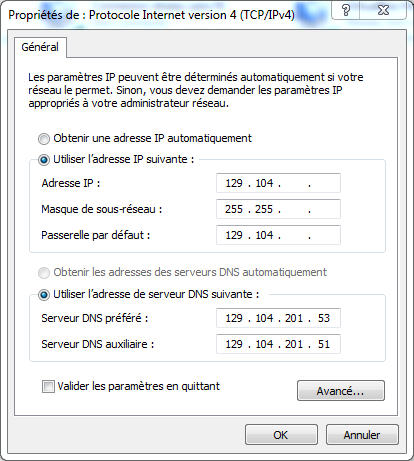
\includegraphics[width=0.48\textwidth]{images/win_config_ip} \label{config:win:IP1}}
%      \hspace{\stretch{1}}
%      \subfloat[Configuration DNS]{ 
%         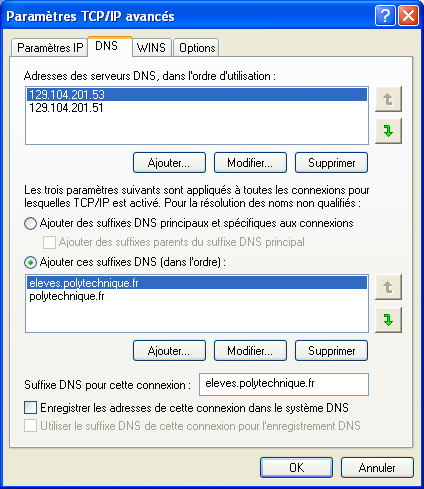
\includegraphics[width=0.48 \textwidth]{images/win_config_dns2} \label{config:win:IP2}}
%             \caption{Configuration réseau}
%    \end{center}
%  \end{figure*}
%
%
%
%%% \newpage
%Coche alors les cases \menu{Utiliser l'adresse IP suivante} et \menu{Utiliser l'adresse de serveur DNS suivante} et remplis les cinq champs d'adresse IP. Tu trouveras toutes les valeurs d'adresse IP nécessaires pour la configuration en page~\pageref{tableau:mon_IP} ; aide-toi de la capture d'écran~\ref{config:win:IP1} pour les placer. Si une partie d'adresse IP est blanche sur cette capture, c'est qu'elle t'est personnelle et que tu dois la calculer !
%Clique ensuite sur le bouton \menu{Avancé}, puis sur l'onglet
%\menu{DNS} en haut.
%Il n'y a plus qu'à  remplir les différents champs comme sur la
%capture d'écran suivante, avec le bouton \menu{Ajouter} et les
%flèches pour réordonner les éléments.
%
%
%%\subsubsection{Le domaine Windows}
%
%%\paragraph{Qu'est ce que c'est ?}
%%Le domaine Windows est un système d'automatisation de la
%%configuration de plusieurs ordinateurs sous Windows situés sur le
%%même réseau. En fait, c'est un outil d'administration, conçu par
%%exemple pour des entreprises où un service informatique doit gérer
%%de nombreuses machines; il permet d'appliquer des modifications de
%%configuration à  toutes les machines du domaine directement depuis un
%%serveur. Le BR possède un serveur dédié au domaine Windows,
%%\server{enez}.
%
%%Le domaine met à  jour automatiquement Windows et l'antivirus à  partir d'\server{enez} (très rapide car tu n'as pas besoin de récupérer des fichiers
%%en dehors de l'école!). Il configure le \emph{firewall} (pare-feu: système de protection contre les éventuelles attaques par le réseau) Windows, mais
%%il est toujours possible de le désactiver si tu préfères un autre \emph{firewall}. En bref, il permet de simplifier à  l'extrême %la mise à  jour
%%continuelle de l'ordinateur.%
%
%
%%\paragraph{Alors, domaine ou pas domaine ?} Soit tu choisis de te
%%mettre sur le domaine Windows, et tu vas alors au paragraphe
%%\guillemotleft~Inscription sur le domaine Windows~\guillemotright.%
%
%%% \newpage
%%\textbf{Avantages :}
%%\begin{itemize}
%%\item Windows est mis à  jour automatiquement ; tu as toujours les
%%dernières corrections de sécurité et un pare-feu correctement
%%configuré. Donc tu es mieux protégé contre les intrusions.
%%\item Surtout, tu n'as plus à  t'en occuper, presque tout est automatique.
%%\end{itemize}%
%
%%\textbf{Inconvénients :}
%%\begin{itemize}
%%  \item Tu délègues une partie des droits d'administration de ta machine au BR
%%        (tout ce qui concerne la sécurité du réseau en particulier).
%%        Cependant, si tu ne sais pas le faire, c'est plutôt un avantage
%%        de laisser le BR s'en occuper à  ta place.
%%  \item Cela ne marche qu'avec Windows 2000, Windows XP Pro ou Windows Vista Business.
%%        On te rappelle que tu peux facilement, gratuitement et légalement passer à 
%%        Windows XP Pro ou bien à  Windows Vista Business (section sur les licences
%%        MSDNAA en page \pageref{msdnaa}).
%%\end{itemize}
%
%%Bien s\^{u}r, tu peux sortir du domaine à  tout instant, et effectuer manuellement les réglages nécessaires à  la sécurité de ton ordinateur.
%
%%Soit tu choisis de configurer toi-même ton ordinateur, et tu peux passer
%%directement à  la section \guillemotleft Installation de l'antivirus
%%\guillemotright. Tu trouveras les informations nécessaires à  la configuration
%%manuelle du pare-feu et du proxy pour \app{Windows Update} en annexe à  la
%%fin de cette section, en page \pageref{horsdomaine}.
%
%%\textbf{Avantage :} Tu es le seul à  t'occuper de la gestion de ton ordinateur.
%
%%\textbf{Inconvénient :} Tu es le seul à  t'occuper de la gestion de ton ordinateur. ;-)
%%S'il devient un foyer pour virus, sache que nous avons les moyens de l'isoler
%%pour éviter toute propagation.
%
%%\begin{center}
%%  \fbox{
%%    \begin{minipage}{.7\textwidth}
%%      \begin{center}
%%Le BR te conseille \emph{très fortement} de te mettre sur le domaine
%%et de choisir l'installation simplifiée !
%%      \end{center}
%%    \end{minipage}
%%  }
%%\end{center}
%
%
%%\paragraph{Inscription sur le domaine Windows}
%
%%On te rappelle que tu ne peux t'inscrire sur le domaine que si tu utilise
%%Windows 2000, Windows XP Pro ou Windows Vista. Si tu possède Windows XP
%%Familial, Windows Vista Home ou encore une version antérieure de Windows,
%%tu dois effectuer toi-même tes réglages de pare-feu et de proxy
%%\app{Windows Update}. Réfère-toi pour cela à  l'annexe ad hoc à  la fin de
%%cette section, en page \pageref{horsdomaine}.
%
%%La procédure d'inscription est la suivante :
%%\begin{itemize}
%
%%\item \textbf{Sous Windows XP :} Clique sur le \menu{Menu Démarrer} puis fais un clic-droit sur
%%\menu{Poste de travail} et choisis \menu{Propriétés}. Ensuite, sélectionne l'onglet \menu{Nom de l'ordinateur} et clique le bouton \menu{Modifier}.
%
%%\item \textbf{Sous Windows Vista :} Clique sur \menu{Menu Démarrer}, puis fais un clic-droit sur \menu{Ordinateur}, \menu{Propriétés}. Là  sélectionne \menu{Paramètres système avancés}, onglet \menu{Nom de l'ordinateur}, puis clique sur le bouton \menu{Modifier}.
%
%%\end{itemize}
%
%%Dans la case \menu{Nom de l'ordinateur}, rentre ton pseudo, puis coche la case \menu{domaine} et
%%rentre \urllink{windows.eleves.polytechnique.fr}. Note bien que l'inscription au domaine te sera
%%refusée par le serveur si quelqu'un d'autre utilise déjà  le même nom d'ordinateur que toi. Par
%%conséquent, essaie d'opter pour un pseudo qui t'identifie de façon claire et unique, par exemple
%%\cmd{NOM\_PRENOM} \footnote{Les Jean Dupont et les Julien Thomas sont priés de trouver autre chose
%%;-)}.
%
%%\imagepos{images/win_config_domaine}{0.5}{S'inscrire sur le domaine windows}{!ht}
%
%%\begin{center}
%%\begin{tabular}{ll}
%% \parbox{.45\textwidth}{
%%  et si tu es rouje 2006 :
%%  \begin{description}
%%    \item[Nom] rouje06
%%    \item[Mot de passe] rouje.2006
%%  \end{description}
% % }
%% & \parbox{.45\textwidth}{
%%  Si tu es jône 2007, tu rentres :
%%  \begin{description}
%%    \item[Nom] jone07
%%    \item[Mot de passe] jone.2007
%%  \end{description}
%%  }
%%\\
%%\end{tabular}
%%\end{center}
%
%%\emph{Attention, ces identifiants servent juste à  t'inscrire sur le
%%domaine. Pour utiliser ton ordinateur, tu devras rentrer au
%%démarrage les mêmes nom d'utilisateur et mot de passe que tu avais
%%avant d'être sur le domaine !}
%%
%%
%%
%%%\paragraph{Installation personnalisée} --- configuration manuelle
%
%%\subparagraph{Configuration antivirus} Le BR, concerné par la
%%sécurité du réseau, te propose un antivirus pour lequel tu n'auras
%%pas à  payer la license pour obtenir les mises à  jour. Bien sà�¿½r,
%%libre à  toi d'utiliser ton anti-virus personnel ; cependant il sera
%%à  ta charge de le mettre à  jour très réguliérement. Pour cela
%%utilise comme proxy : \urllink{http://kuzh} sur le port 8080.
%
%%\emph{Installation de l'anti-virus du BR}\ : Commence par
%%désinstaller tous les antivirus ou firewalls que tu pourrais avoir
%%comme expliqué dans le paragraphe \guillemotleft~Installation simplifiée
%%--- configuration automatique~\guillemotright .
%
%%Puis ouvre ton explorateur Windows et tape :
%%\urllink{$\backslash\backslash$enez$\backslash$antivirus}
%%et double-clique sur le fichier \file{Symantec.exe}.
%
%%Ce package contient le paramétrage de la mise à  jour automatique de
%%Windows sur le serveur de l'école. Attends la fin de l'installation
%%et c'est fini ! Maintenant, tu n'as plus à  toucher à  l'antivirus,
%%normalement il sera mis à  jour automatiquement.
%
%%\subparagraph{Configuration firewall}
%
%%Si tu as Windows XP avec le SP2 installé, tu as un firewall
%%automatiquement activé et facile d'utilisation. En effet, à  chaque
%%fois qu'un programme tentera d'aller pour la première fois sur
%%Internet, il te demandera si tu veux le laisser faire ou non, comme
%%dans la capture~\ref{config:win:firewall}.
%
%%\imageref{images/win_firewall}{0.8}{Un programmme --- ici GuildFTP
%%--- demande à  accéder au réseau}{!ht}{config:win:firewall}
%
%%Le firewall commercial \app{ZoneAlarm}, indépendant de Windows,
%%fonctionne sur le même principe. Tu peux le trouver sur \xshare.
%
%%Si tu préfères utiliser le firewall intégré à  Windows XP (sans le
%%SP2) ou à  Windows Server 2003, il te faudra le configurer en détail.
%%Va dans le \menu{Menu Démarrer}, \menu{Paramètres} et clique sur
%%\menu{Connexions Réseau}. Choisis la connexion qui est utilisée par
%%ton ordinateur (souvent il n'y en a qu'une, ou alors une seule est
%%activée) et double-clique dessus. Clique sur \menu{Propriétés} en
%%bas à  gauche, puis sur l'onglet \menu{Avancé} et rentre dans le menu
%%de \menu{Paramètres} du \menu{Pare-feu Windows}. Il te faudra alors
%%ajouter manuellement tous les ports que tu veux ouvrir sur
%%l'extérieur. Pour cela, clique sur \menu{Ajouter}, et remplis la
%%boà�¿½te de dialogue en t'aidant de la capture
%%d'écran~\ref{config:win:ouvrir_port}; mets le numéro du port que tu
%%veux ouvrir, par exemple 5050, 5053 et 5055 en TCP pour \app{qRezix}
%%et 21 en TCP pour ton FTP.
%
%%\imageref{images/win_config_firewall}{0.7}{Ouvrir un port dans le firewall %Windows}{!ht}{config:win:ouvrir_port}
%
%%Comme tu peux le constater, il est beaucoup plus pratique d'aller
%%sur le domaine et de laisser le SP2 faire le gros du boulot à  ta
%%place :-).
%
%
%
%\subsubsection{Configuration \emph{web} (serveur mandataire)}
%
%\imageref{images/win_config_proxy}{0.5}{Configuration du serveur mandataire (\emph{proxy})}{!ht}{config:win:proxy}
%
%Même si tu n'utilises pas \app{Internet Explorer} comme client \emph{web}, Windows et d'autres programmes
%utilisent ses paramètres, notamment \app{Windows Update}. Par conséquent lance \app{Internet Explorer} et va
%dans le menu \menu{Outils}, \menu{Options Internet}, puis sur l'onglet \menu{Connexions} de la
%nouvelle fenêtre et enfin sur \menu{Paramètres réseau} dans le bas de la fenêtre. Tu dois être arrivé sur une fenêtre semblable à celle de la capture d'écran~\ref{config:win:proxy}. Là, coche
%uniquement la case \menu{Utiliser un script de configuration automatique}, puis remplis le champ
%\menu{Adresse} avec \urllink{http://config/proxy.pac}.
%
%Une fois que tu as fait ça, tu n'as plus forcément besoin d'\app{Internet Explorer}, tu peux donc utiliser un autre navigateur, comme \app{Mozilla
%Firefox}, disponible sur \urllink{http://www.mozilla-europe.org/fr/products/}.
%
%Même si tu ne configures pas Windows Update avec le paragraphe ci-dessous, n'oublie pas de régler ton navigateur \emph{web} et ton client \emph{mail} si tu en as un : reporte-toi page \pageref{browser}.
%
%\subsubsection{Windows Update}
%
%\label{horsdomaine} %\emph{Cette sous-section ne concerne pas les gens qui ont choisi de s'inscrire sur le domaine.}
%
%%\paragraph{Pare-feu} Si tu as Windows XP avec le SP2 installé, ou \emph{a fortiori}
%%Windows Vista, tu as un \emph{firewall} automatiquement activé et facile d'utilisation. En effet, à  chaque fois qu'un programme tentera d'aller pour
%%la première fois sur Internet, il te demandera si tu veux le laisser faire ou non. Si tu préfères une protection indépendante de Windows, le
%%\emph{firewall} commercial \app{Zone\-Alarm} fonctionne sur le même principe. Tu peux le trouver sur \xshare.
%
%%Si tu préfères utiliser le \emph{firewall} intégré à  Windows XP (sans le SP2), il te faudra le configurer en détail. Va dans le \menu{Menu Démarrer},
%%\menu{Paramètres} et clique sur \menu{Connexions Réseau}. Choisis la connexion qui est utilisée par ton ordinateur (souvent il n'y en a qu'une, ou
%%alors une seule est activée) et double-clique dessus. Clique sur \menu{Propriétés} en bas à  gauche, puis sur l'onglet \menu{Avancé} et rentre dans le
%%menu de \menu{Paramètres} du \menu{Pare-feu Windows}. Il te faudra alors ajouter manuellement tous les ports que tu veux ouvrir sur l'extérieur. Pour
%%cela, clique sur \menu{Ajouter}, et remplis la boîte de dialogue% en t'aidant de la capture d'écran~\ref{config:win:ouvrir_port} ci après
%%; mets le numéro du port que tu veux ouvrir, par exemple 5050, 5053 et 5055 en TCP pour \app{qRezix} et 21 en TCP pour ton FTP.
%
%Il reste une dernière configuration de
%serveur mandatataire indispensable pour que puissent se faire les mises à  jour automatiques
%de Windows. Il t'est fortement recommandé de le faire.
%
%\begin{description}
%
%\item[Sous Windows 7 \& Windows 8] Si tu as correctement configuré ton serveur \emph{web} mandataire, les mises à jours se font automatiquement.
%
%\item[Sous Windows XP] Fais \menu{Démarrer}, \menu{Exécuter}, puis
%tape \cmd{cmd} dans la fenêtre qui s'affiche. Une ligne de commande apparaît,
%il te suffit alors de taper : \cmd{proxycfg -p http://kuzh:8080} pour régler
%le serveur mandataire. Pour revenir à  un accès direct il faut taper \cmd{proxycfg -d}.
%
%\item[Sous Windows Vista]
%Dans le menu \menu{Démarrer}, tape \guillemotleft~Invite de commandes~\guillemotright{} dans le champ \menu{Rechercher}, puis clique droit sur le lien
%et choisis \menu{Exécuter en tant qu'administrateur}. Tape ensuite les commandes suivantes :
%\cmdline{
%C:\textbackslash{}Windows\textbackslash{}system32$>$netsh\\
%netsh>winhttp\\
%netsh winhttp>set proxy proxy-server="http://kuzh:8080"\\
%netsh winhttp>exit\\
%C:\textbackslash{}Windows\textbackslash{}system32>exit }
%
%Pour revenir à l'accès direct, il suffit de taper :
%\cmdline{
%  netsh winhttp reset proxy
%}
%
%Pour la suite de ta configuration, rendez-vous page \pageref{browser} pour faire marcher ton navigateur web préféré !
%
%\end{description}

%\clearpage

\markright{Configuration sous Mac OS}
\label{mac} \bghdr{images/fond-mac}

%\begin{center}
%
\includegraphics{images/logo_Mac}
%\end{center}



\subsection{Configuration sous Mac OS X}

La configuration est d\'etaill\'ee pour Mac OS 10.5 (\app{Leopard}). %et encore un peu pour Mac OS 10.4 (Tiger).
Afin de conna\^itre la version que tu utilises, va dans le \menu{menu Pomme} puis s\'electionne \menu{\`A propos de ce Mac}.

\subsubsection{Configuration IP}

\flimage{images/mac_prefs_icone}{0.07}{l}
 \app{Pr\'ef\'erences R\'eseau}, accessible depuis l'article de menu \menu{Pr\'ef\'erences syst\`eme} du menu \menu{Pomme}, permet de configurer la connexion au r\'eseau. Par ailleurs, si au d\'emarrage un assistant te propose de configurer ton r\'eseau, refuse et utilise la proc\'edure du BR. En effet, le r\'eseau n\'ecessite une configuration particuli\`ere  \`a l'X, plus complexe que celle effectu\'ee par cet assistant.


\noindent
  \begin{figure*}[h]
    \begin{center}  
     % \subfloat[Tiger]{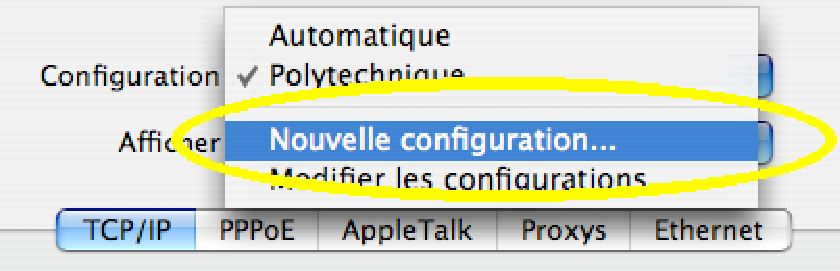
\includegraphics[width=0.47\textwidth]{images/mac_nouvelle_config} } 
     % \hfill
      \subfloat[Cr\'eer une nouvelle configuration r\'eseau]{ 
      \begin{minipage}{0.43 \textwidth}\begin{flushleft}
      {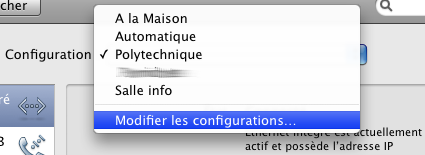
\includegraphics[width=0.96\textwidth]{images/mac_nouvelle_config_leopard_1}}\\ \vspace*{2cm}
      {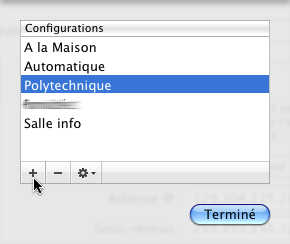
\includegraphics[width=0.96\textwidth]{images/mac_nouvelle_config_leopard_2}} 
 		\end{flushleft}  \end{minipage}
 		 } 		
 		\subfloat[Configuration de l'interface r\'eseau \emph{Ethernet}, de l'adresse IP et du \emph{proxy}]{ 
 		 \begin{minipage}{0.43 \textwidth}\begin{flushright}
 		{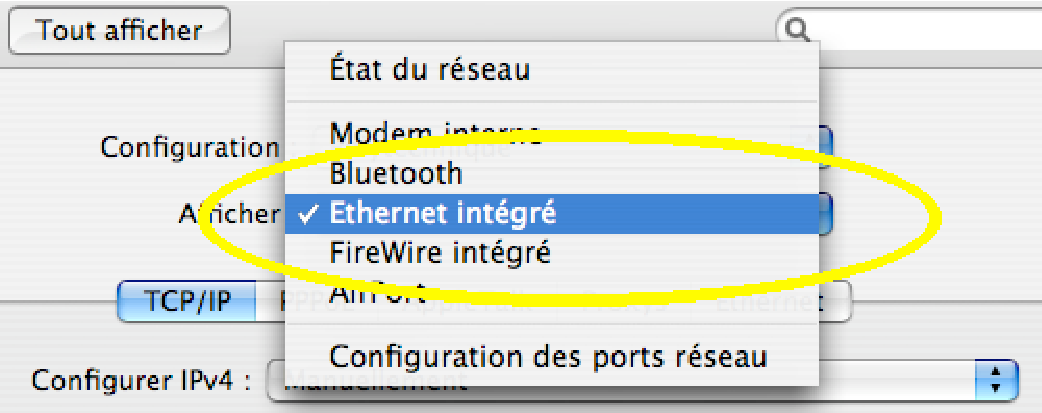
\includegraphics[width=0.96 \textwidth]{images/mac_config_ethernet}} \\ 
 		{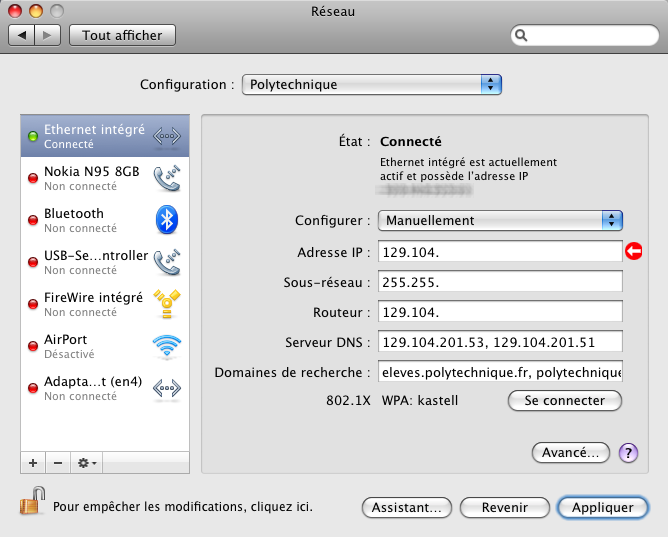
\includegraphics[width=0.96 \textwidth]{images/mac_config_ip_leopard}} \\
 		{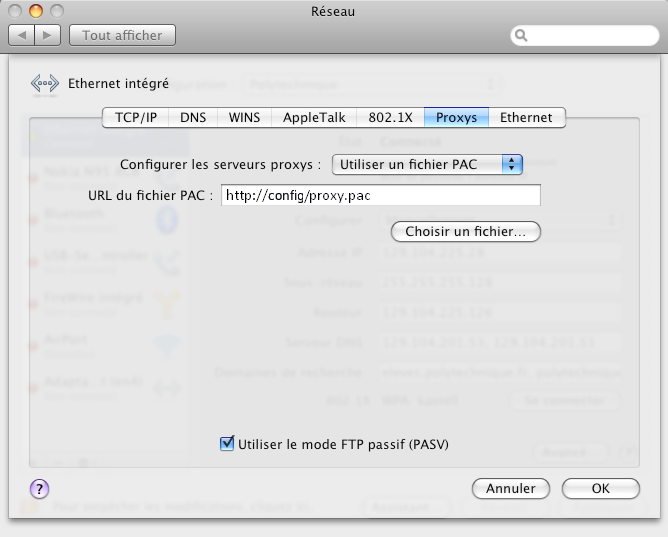
\includegraphics[width=0.96 \textwidth]{images/mac_config_proxy_leopard}}
\end{flushright}
 		\end{minipage}
 		 	\label{config:mac:ip:leopard}	}
     	 \caption{Cr\'eer une nouvelle configuration r\'eseau}

    \end{center}
  \end{figure*}

\pagebreak

La gestion des configurations r\'eseau de Mac OS X permet de cr\'eer plusieurs configurations et de passer en un clic de l'une  l'autre gr\^ace au sous-menu \menu{Configuration R\'eseau} du menu \menu{Pomme}. Cela est tr\`es pratique pour les machines vou\'ees \`a  \^etre connect\'ees \`a  plusieurs endroits successivement --- les portables par exemple (voir la page~\pageref{wifi} puis la section \emph{Wi-Fi} pour plus de pr\'ecisions sur le \emph{Wi-Fi}). Commence donc par cr\'eer une nouvelle configuration r\'eseau dans le menu d\'eroulant \menu{Configuration}.



Une fois la nouvelle configuration cr\'e\'ee, il faut configurer l'interface r\'eseau \emph{Ethernet}.



\app{Leopard} : Dans la colonne de gauche, s\'electionne \menu{Ethernet int\'egr\'e}.

Choisis alors \menu{Configurer IPv4} :% \menu{Manuellement} (\app{Tiger}) ou 
\menu{Configurer} : \menu{Manuellement} (\app{Leopard}). Tu trouveras toutes les valeurs d'adresses IP n\'ecessaires pour la configuration en page \pageref{calcul_ip} ou en te reportant aux captures d'\'ecran~\ref{config:mac:ip:leopard}. Si une partie d'adresse IP est blanche sur ces captures, c'est qu'elle t'est personnelle et que tu dois la calculer !


  
  

%\imageref{images/mac_config_ip_leopard}{0.4}{Configuration IP (Leopard)}{!ht}{config:mac:ip:leopard}}


Pour avoir acc\`es \`a  Internet, il faut aussi configurer le \emph{proxy}.

\app{Leopard} : Clique sur le bouton \menu{Avanc\'e...} puis sur l'onglet \menu{Proxys}.


\app{Mac OS X 10.3.3 et sup\'erieur} :  choisis l'option \menu{Configuration automatique de proxy} et indique http://config/proxy.pac comme URL de fichier PAC. Pour Mac OS X 10.3 \`a  10.3.2, n'oublie pas une fois que tu as le r\'eseau de faire la mise \`a  jour de ton syst\`eme, pour pouvoir configurer de fa\c con automatique le \emph{proxy}.

\app{Mac OS X 10.3.2 et inf\'erieur} : il te faut sp\'ecifier tous les
\emph{proxies} manuellement, et mettre \server{kuzh.polytechnique.fr}, port \server{8080}. Malheureusement, cele te permettra uniquement d'acc\'eder aux sites h\'eb\'erg\'es hors du plat\^al : les sites \'el\`eves ne fonctionneront pas.


N'oublie pas d'activer le mode passif pour les transferts en FTP, en cochant la case comme dans la capture.

\subsubsection{Configuration antivirus}

Bien qu'il soit important de maintenir ton syst\`eme \`a  jour, un antivirus est pour l'instant tout \`a  fait superflu sur Mac, puisqu'aucun virus fonctionnel n'a encore vu le jour. Attention cependant, n'ouvre pas des fichiers dont tu ne te sois pas assur\'e de la provenance, et essaie de te tenir au courant des actualit\'es concernant les failles des applications que tu utilises.

\subsubsection{Configuration web}
\flimage{images/nux_firefox_icon}{0.07}{l}
Un point particulier pour la configuration du \emph{proxy} de \app{Firefox} : dans \menu{Pr\'ef\'erences}, \menu{Avanc\'e}, \menu{R\'eseau}, clique sur \menu{Param\`etres} et, dans le champ \menu{Adresse de configuration automatique du proxy}, inscris : \urllink{http://config/proxy.pac}. 
\\
\\

\flimage{images/mac_safari_icone}{0.07}{l}
\app{Safari}, le navigateur web d'Apple, est maintenant compatible avec la majorit\'e des sites \emph{web}. Tu peux donc t'en servir au quotidien, en faisant appel \`a  \app{Firefox} pour les sites r\'ecalcitrants. Un conseil : pense \`a  activer le blocage des fen\^etres \emph{pop-up} (dans le menu \menu{Safari}). \app{Safari} peut aussi servir de client RSS (voir plus bas).\\
\\

\app{Google Chrome} se règle quant à lui automatiquement sur la configuration du système. 
\\

\subsubsection{Configuration \emph{mail}}
\flimage{images/mac_mail_icone}{0.07}{l} \app{Mail} : un client \emph{mail} offrant les fonctionnalit\'es classiques d'un bon client : recherche instantan\'ee, filtre antispam, r\`egles de tri automatique des \emph{mails}, regroupement des \emph{mails} correspondant \`a  une m\^eme discussion.

Au premier lancement, \app{Mail} te demandera de remplir les informations concernant ton compte \emph{mail} sur \server{poly}, il suffit de le remplir avec les donn\'ees suivantes :
\begin{description}
  \item[Nom complet] ton nom !
  \item[Adresse \'electronique] de la forme \mail{prenom.nom@polytechnique.edu}
  \item[Serveur de r\'eception] \server{poly.polytechnique.fr}
  \item[Type de compte] \menu{POP}
  \item[Nom d'utilisateur] ton \emph{login} \server{poly} (les huit premi\`eres lettres de ton nom en g\'en\'eral)
  \item[Mot de passe] ton mot de passe \server{poly}
  \item[Serveur d'envoi (SMTP)] \server{poly.polytechnique.fr} ou \server{ssl.polytechnique.org}
\end{description}

Si tu as d\'ej\`a  cr\'e\'e un compte pr\'ec\'edemment, il faut aller dans les \menu{Pr\'ef\'erences} (accessibles depuis le menu \menu{Mail}), onglet \menu{Comptes}, pour cr\'eer un autre compte en cliquant sur la case \menu{+}.

N'oublie pas de cocher \menu{Activer le cryptage SSL} dans l'onglet \menu{Avanc\'e}, port 995. Tu souhaiteras alors certainement installer le certificat de s\'ecurit\'e de \server{poly} (tu le trouveras sur \urllink{http://poly/}). Une fois que tu as t\'el\'echarg\'e le certificat, ouvre le fichier \menu{.CRT} obtenu, et dans \app{Trousseau d'acc\`es}, installe-le dans %\menu{X509Anchors} (Tiger) ou 
\menu{session} (Leopard).

Cette configuration marche pour acc\'eder \`a  ses mails depuis l'int\'erieur de l'X mais aussi de l'ext\'erieur, sans rien changer. En revanche tu ne peux pas envoyer de \emph{mails} depuis l'ext\'erieur , car le serveur \server{poly} ne le permet pas. Nous te conseillons vivement d'utiliser le serveur SMTP \server{polytechnique.org} et de regarder la configuration propos\'ee par \urllink{Polytechnique.org}. Celle-ci permet d'envoyer des \emph{mails} s\^urs \`a  l'ext\'erieur de l'\'Ecole sans modifier ta configuration par la suite. Tu peux ajouter ce SMTP dans l'onglet \menu{Comptes} des \menu{Pr\'ef\'erences} de \emph{mail} et r\'egler dans l'onglet \menu{Avanc\'es} comme dans la capture.

\begin{figure*}[!hl]
    \begin{center}
	      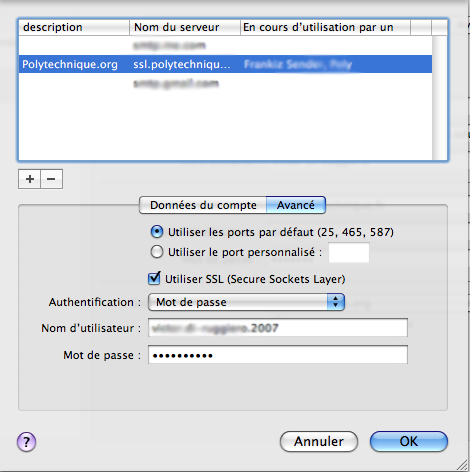
\includegraphics[width=0.4\textwidth]{images/mac_config_smtp_poltechnique.png} 
      \caption{Configurer le serveur SMTP \server{Polytechnique.org}}
    \end{center}
  \end{figure*}

Le LDAP ne fonctionne pas \`a  l'heure actuelle avec \app{Mail} (mars 2009) sous \app{Leopard}, contrairement aux  autres syst\`emes d'exploitation (fonctionne cependant avec \app{Thunderbird}).
%\subsuEnfin, tu peux disposer dans \app{Mail} de l'annuaire de l'\`acole, mis \`a  disposition par la DSI. Pour cela, va dans les \menu{Pr\'ef\'erences} de Mail,
%puis dans la rubrique \menu{R\'edaction} et clique sur \menu{Configurer LDAP\ldots}. Tu peux ensuite utiliser le bouton \menu{+} pour ajouter un
%serveur, et remplir la fen\^etre comme sur la capture.

%\imagepos{images/mac_config_ldap}{0.6}{Configurer l'annuaire}{!ht}
%bsection{Logiciels additionnels}

Les logiciels suivants sont utiles pour utiliser avec Mac OS X les services propos\'es sur le r\'eseau ; ils sont t\'el\'echargeables sur \server{frankiz}, dans la rubrique \menu{T\'el\'echarger}, \menu{Mac}.

%\subsubsection{Configuration \emph{news}}
%
%\flimage{images/mac_thunderbird_icone}{0.07}{l} 
%\app{Thunderbird} : un client \emph{news} permettant d'acc\'eder aux forums de discussion des \'el\`eves (voir page~\pageref{newsgroups} pour les d\'etails sur \server{frankiz}), mais aussi \`a  ceux de \server{usenet} gr\^ace au serveur \server{polynews.polytechnique.fr}. Il est tr\`es proche d'\app{Outlook Express} dans son esprit. Dans la m\^eme cat\'egorie, il existe \app{MacSOUP}, \app{Unison} ou encore \app{MT-NewsWatcher}. La configuration se fait de la m\^eme mani\`ere.
%
%Au premier lancement, l'application te propose d'importer les param\`etres depuis une autre application. Clique sur \menu{Suivant}. Tu peux alors choisir quel type de compte tu veux configurer (tu remarqueras que tu peux aussi cr\'eer un compte courrier \'electronique, et un compte RSS). S\'electionne \menu{Compte forums de discussion} et clique sur \menu{Suivant}. Entre alors les informations suivantes :
%
%\begin{description}
%  \item[Votre nom] ton nom ou ton pseudo
%  \item[Adresse de courrier] \mail{prenom.nom@polytechnique.edu}
%  \item[Serveur de forums] \server{news}
%  \item[Nom du compte] News Frankiz
%  \item[Nom d'utilisateur] ton \emph{login }poly (les huit premi\`eres lettres de ton nom en g\'en\'eral)
%  \item[Serveur d'envoi (SMTP)] \server{poly.polytechnique.fr} ou \server{ssl.polytechnique.org}
%\end{description}
%
%
%Pour t'abonner \`a  des groupes de discussion, il te suffit de s\'electionner le compte \menu{News Frankiz} dans la fen\^etre \menu{Dossiers} de \app{Thunderbird}, puis de cliquer sur \menu{G\'erer les abonnements aux groupes de discussion}. Tu pourras ensuite s\'electionner les forums qui t'int\'eressent parmi la liste propos\'ee. Reporte-toi \`a  la page \pageref{newsgroups} pour plus d'infos sur les \emph{newsgroups} auxquels t'abonner !
%

\subsubsection{Autres logiciels utiles}

%\flimage{images/mac_qrezix_icone}{0.07}{l} \app{qRezix} : en deux mots, c'est un programme d\'evelopp\'e par le BR pour faciliter la vie sur le r\'eseau. Tu peux le r\'ecup\'erer via le lien qRezix sur \server{Frankiz} ou sur \urllink{http://br.frankiz.net/qrezix/mac/}. Pour plus de d\'etails, voir le paragraphe consacr\'e \`a  qRezix \`a  la page \pageref{qrezix}. \\

%\app{Leopard} : le pare-feu se r\`egle pour chaque application; tu n'auras qu'\`a  r\'epondre \menu{Autoriser} lorsqu'il te demandera si tu veux \menu{Autoriser les connexions entrantes}.

%\noindent  \app{Tiger} : Attention, si ton \emph{firewall} est activ\'e, tu dois ouvrir les ports 5050, 5053 et 5055 en TCP. Pour cela va dans \app{Pr\'ef\'erences Syst\`eme}, dans le module \menu{S\'ecurit\'e}, onglet \menu{Coupe-feu}. S'il est \'ecrit \menu{Coupe-feu activ\'e}, clique le bouton \menu{Nouveau} et remplis la bo\^ite de dialogue comme sur la capture d'\'ecran ci-dessous pour ouvrir les ports.

%\imagepos{images/mac_firewall}{0.5}{Ouvrir les ports pour \app{qRezix} (Tiger)}{!ht}

%\flimage{images/mac_conversation_icone}{0.1}{l}
%\noindent\app{Colloquy}, un client IRC dans le m\^eme esprit qu'\app{iChat}. Il dispose d'une interface tr\`es simple ne n\'ecessitant pas de conna\^itre les commandes IRC. Tu peux te reporter \`a  la page \pageref{irc} pour plus d'infos sur l'IRC. \app{X-Chat Aqua} est un autre client IRC, plus riche en fonctionnalit\'es, mais moins agr\'eable \`a  utiliser. \\

%\flimage{images/mac_netnewswire_icone}{0.1}{l}
%\noindent\app{NetNewsWire} est la r\'ef\'erence des clients RSS sur Mac, et est maintenant gratuit. Dans le m\^eme genre, on peut citer \app{Vienna}, un client RSS open source, dont le d\'eveloppement actif est prometteur. Les flux RSS permettent d'agr\'eger dans un seul logiciel des informations en provenance de nombreux sites web, qui peuvent provenir de forums de discussions, de mises \`a  jour de logiciels, d'informations internationales\dots \\ \\

%\flimage{images/mac_fink_icone}{0.07}{l} \app{Fink} est la mani\`ere la plus simple d'installer sur Mac OS X nombre de logiciels issus du monde Unix (Linux par exemple). Gr\^ace \`a  lui, tu pourras installer les m\^emes logiciels que dans les salles informatiques. Par exemple, tu pourras installer Scilab sans trop de peine\dots La configuration n\'ecessaire se trouve sur la page \urllink{http://frankiz/binets/reseau/Miroir\_Fink}.\\ 

\flimage{images/logo_Windows}{0.1}{l}
 \app{Windows et les Mac Intel} : Maintenant il est possible d'installer Windows gr\^ace \`a  \app{Boot Camp}, livr\'e avec \app{Leopard}. Cela te permettra de profiter des quelques applications du monde PC qui valent le coup tout en gardant ton Mac. Tu peux \'egalement virtualiser Windows (utiliser Windows en utilisant en m\^eme temps Mac OS) gr\^ace \`a  \app{VMware Fusion}, \app{VirtualBox} ou \app{Parallels Desktop}. Le  d\'efaut de cette solution est que tu n'as pas d'acc\'el\'eration 3D, donc pour les jeux il te faudra red\'emarrer. Ces trois logiciels sont disponibles sur leurs sites \emph{web} respectifs. \`A toi de choisir !
Mais v\'erifie tout de m\^eme que tu as bien un processeur Intel (\menu{Pomme} puis s\'electionne \menu{\`A propos de ce Mac}).

\clearpage


\markright{Configuration sous Linux}
\label{ubuntu} %$Id: config_nux.tex 145 2005-03-25 08:26:35Z myk $

\bghdr{images/fond_ubuntu}



%\begin{center}
%
\includegraphics{images/logo_Linux}
%\end{center}

\subsection{Configuration sous Ubuntu/Kubuntu}

Cette section décrit la configuration de ta connexion Internet sous Ubuntu GNU/Linux (ou une de ses variantes). Pour les autres distributions, tu peux adapter les instructions ci-dessous ou consulter la version 
en ligne de commande, page \pageref{linux_cmdline}.

\subsubsection{Configuration IP}
Tu as besoin de conna\^itre ton adresse IP, ton masque de sous-r\'eseau et ta  passerelle. Toutes les informations se trouvent page \pageref{calcul_ip}. Bien s\^ur, pour  l'ensemble des manipulations d\'ecrites ci-dessous tu auras besoin de ton  mot de passe super-utilisateur (\emph{root}) !

\label{Ubuntu:IP}
Il existe deux mani\`eres de configurer tes param\`etres r\'eseaux: l'une utilise les outils graphiques de l'environnement que tu as choisi (Gnome ou KDE), 
l'autre utilise simplement la ligne de commande. Bien sûr, les outils graphiques ne sont qu'un interm\'ediaire modifiant les fichiers dont on te parle 
plus bas. Ils te permettent parfois d'enregistrer une configuration r\'eseau, ce qui facilite la gestion si tu rentres souvent chez toi. Pour obtenir le 
m\^eme r\'esultat en ligne de commande il faut utiliser un script.
\begin{description}
\item[\'Etape 1 : configuration de la connexion au r\'eseau] \
 
\begin{itemize}
\item Va dans \menu{Syst\`eme}, \menu{Pr\'ef\'erences} puis \menu{Connexions r\'eseau}.
\item Dans l'onglet \menu{Filaire}, clique sur \menu{Ajouter}.
\item Compl\`ete le champ \menu{Nom de la connexion}  par ce que tu veux ; "Casert de Polytechnique" par exemple.
\item Puis va dans l'onglet \menu{Param\`etres IPv4}.
\item S\'electionne la m\'ethode \menu{Manuel}.
\item Clique sur \menu{Ajouter}, puis remplis les champs \menu{Adresse}, \menu{Masque de r\'eseau} et  \menu{Passerelle} par les donn\'ees qui te sont propres. 
\item Compl\`ete le  champ \menu{Serveurs DNS} par \server{129.104.201.53, 129.104.201.51} et le champ \menu{Domaines de recherche} par \server{eleves.polytechnique.fr, polytechnique.fr}. 
\item Coche enfin l'option \menu{Disponible pour tous les utilisateurs}, clique sur \menu{Appliquer} et enfin rentre ton mot de passe super-utilisateur (root).
\end{itemize}

\item[\'Etape 2 : configuration du proxy (= serveur mandataire)] \
\begin{itemize}
\item Va  dans \menu{Param\`etres Syst\`eme}, \menu{R\'eseau} puis \menu{Serveur Mandataire}.
\item S\'electionne  la \menu{M\'ethode} \menu{Automatique}.
\item Compl\`ete le champ  \menu{URL de configuration} par \urllink{http://config/proxy.pac}. 
\item Clique sur \menu{Appliquer à tout le syst\`eme...} et rentre ton mot de passe super-utilisateur si on te le demande.
\end{itemize}

\item[\'Etape 3 (\'eventuellement)] \
\begin{itemize}
\item Clique  sur l'ic\^one de l'applet R\'eseau dans la zone de notification, en forme  de fl\`eches t\^ete-b\^eche ou d'ondes. S\'electionne le r\'eseau que tu as  configur\'e dans la 1\`ere \'etape, et te voilà connect\'e à Internet !
\item Une fois ta configuration r\'eseau termin\'ee, tu peux la tester en \emph{pinguant} \fkz (dans une console), o\`u tu devrais voir quelque chose comme :
\end{itemize}

\cmdline{\$ ping frankiz\\
PING frankiz.eleves.polytechnique.fr (129.104.201.51) 56(84) bytes of data.\\
64 bytes from Frankiz.eleves.polytechnique.fr ...}

\end{description}



\subsubsection{Configuration du gestionnaire de paquets}
\label{ubuntu_mirror}

Il faut d\'esormais configurer le gestionnaire de paquets pour qu'il utilise les miroirs du BR et non les miroirs à l'ext\'erieur du campus, qui sont plus lents. \
Va  dans \menu{Applications}, \menu{Logith\`eque Ubuntu} puis menu \menu{\'edition}, \menu{Sources de logiciels...}. 
Entre ton  mot de passe super-utilisateur puis s\'electionne l'onglet \menu{Autres  logiciels}. 
D\'ecoche les cases comprenant une adresse du type \urllink{http://archive.canonical.com/ubuntu version}, o\`u \textit{version} correspond à la version d'Ubuntu install\'ee sur ton ordinateur. 
À l'impression de l'InfoBR, la version actuelle est \textbf{oneiric} et la pr\'ec\'edente est \textbf{natty}. \
Clique sur \menu{Ajouter}, puis entre dans le champ \menu{Ligne APT} :
\cmdline{deb ftp://miroir/linux/ubuntu version main restricted universe multiverse}
Tu auras bien s\^ur remplac\'e \textit{version} par ta version d'Ubuntu (\textit{maverick}/\textit{lucid}/\textit{karmic}/...). \\
Clique ensuite sur \menu{Ajouter une source de mise à jour}. Fais de même pour les lignes suivantes :
\cmdline{deb ftp://miroir/linux/ubuntu version-updates main restricted universe  multiverse \\
deb ftp://miroir/linux/ubuntu version-security main restricted universe  multiverse}
Tu peux aussi utiliser le d\'ep\^ot suivant mais attention il contient des logiciels non support\'es par Canonical, l'\'equipe de d\'eveloppement d'Ubuntu (en particulier il peut arriver que certains logiciels contiennent des erreurs) :
\cmdline{deb ftp://miroir/linux/ubuntu version-backports main restricted universe multiverse}
Le  BLL (Binet Logiciels Libres) dispose par ailleurs d'un miroir  non-officiel qui contient des paquets (flash, ...) non  inclus dans la distribution de base pour diverses raisons, en paticulier l\'egales ou \'ethiques. Pour en profiter, rajoute aussi la ligne :
\cmdline{deb ftp://miroir/linux/bll version main}
Clique enfin sur \menu{Fermer} puis r\'eponds \menu{Actualiser} à la fenêtre de dialogue qui appara\^it. \\

Note : il n'est pas n\'ecessaire de configurer Synaptic dans ses Pr\'ef\'erences pour y sp\'ecifier un proxy quelconque.

\subsubsection{Configuration antivirus}

{C'est pas non plus comme si y'en avait besoin \dots}

%\subsubsection{Configuration du pare-feu}
%
%La solution la plus simple pour se faire un \emph{firewall} sous linux est d'utiliser les \emph{iptables}. Pour ceci la premi\`ere \'etape est
%d'installer le paquet \app{iptables} pour ta distribution. Pour savoir comment configurer ton \emph{firewall} pour le r\'eseau de l'X, consulte le Wikix.

\clearpage


\markright{Pour bien commencer}
\bghdr{images/fond-infobr}

\subsection{Configuration de ton navigateur Web}
\label{browser}

\paragraph{Firefox}
\flimage{images/firefox-logo}{0.07}{l}

Lance \app{Mozilla Firefox}, et va dans le menu \menu{Outils},
\menu{Options...} (ou \menu{\'Edition}, \menu{Préférences...} sous Linux.) L\`a , s\'electionne la rubrique \menu{Avanc\'e}, onglet \menu{R\'eseau}, et clique sur
\menu{Param\`etres}. La case \`a  cocher est alors \menu{Adresse de configuration automatique du proxy},
et l'adresse \`a  indiquer est : \urllink{http://config/proxy.pac}.

Ensuite, il te faut acc\'epter le certificat SSL du BR. Cela consiste \`a indiquer que tu fais confiance au BR pour authentifier les sites des binets.\\
Il suffit se se rendre sur \urllink{http://config/ca-br.crt} et de cocher toutes les cases.\\

\noindent
  \begin{figure*}[!h]
    \begin{center}  
      \subfloat[Configuration du serveur mandataire]{ 
      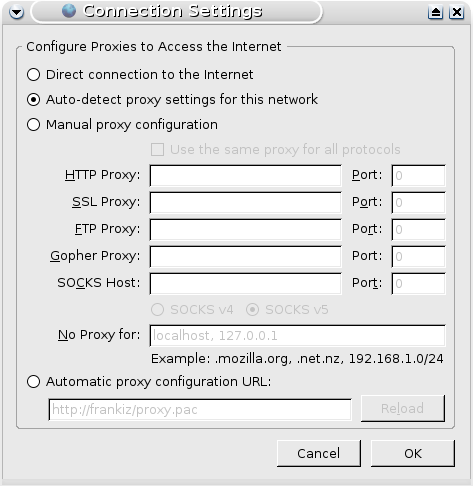
\includegraphics[width=0.48\textwidth]{images/nux_proxy_firefox}}
      \hspace{\stretch{1}}
      \subfloat[Acceptation du certificat BR]{ 
         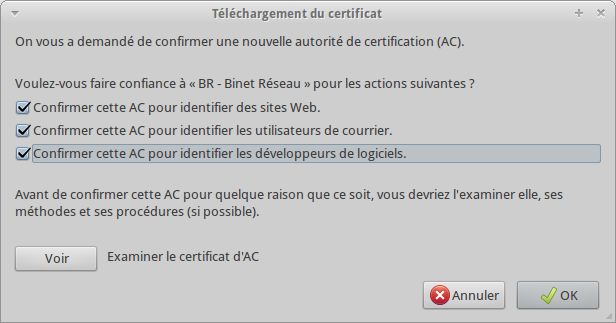
\includegraphics[width=0.48 \textwidth]{images/ca-br-ff}}
           \caption{Configuration de firefox}
    \end{center}
  \end{figure*}
%\imagepos{images/nux_proxy_firefox}{0.65}{Configuration du serveur mandataire sous Firefox}{ht}\\
%\imagepos{images/ca-br}{1}{Acceptation du certificat BR}{ht}
%
% Pour le RTFIBRp11 pour un saut de page si n\'ec\'essaire ce qui n'\'etait pas le cas en 2008

%\noindent\rule{.4\textwidth}{.4pt}

%\vfill %\pagebreak


\paragraph{Google Chrome}
\flimage{images/google-chrome-logo}{0.07}{l}

Pour \app{Google Chrome}, la configuration du serveur mandataire se r\`egle automatique sur celle du système. Tu n'es donc pas obligé de régler le proxy toi-même. Cependant, pour le faire manuellement, clique sur la
clef à molette en haut à droite, choisis \menu{Options}, va dans l'onglet \menu{Paramètres avancés} (ou \menu{Under the Hood}), clique sur \menu{Modifier les paramètres du Proxy...} et règle comme ci-dessus.\\

Pour accepter le certificat BR, il te faut d'abord le t\'el\'echarger sur \urllink{http://config/ca-br.crt}. Puis, dans Chrome, rends toi dans \menu{Pr\'eferences}, \menu{Options avancées}, \menu{G\'erer les certificats}i, \menu{Autorit\'es} et clique sur \menu{Importer}. Il suffit alors de s\'electionner l'emplacement o\`u tu avais stock\'e le certificat et de cocher toutes les cases.
\imagepos{images/ca-br-chrome}{1}{Acceptation du certificat BR}{ht}

\paragraph{Konqueror}
\flimage{images/konqueror-logo}{0.07}{l}

Sous \app{Konqueror}, cela se trouve dans le menu \menu{Configuration}, \menu{Configurer Konqueror},
dans l'onglet \menu{Serveur mandataire} ; ensuite, choisis les même réglages que pour \app{Firefox} ci-dessus. \emph{Attention}: si tu ne configures pas le serveur mandataire dans Konqueror,
les logiciels KDE (\app{KGet}, \app{Adept},\dots) ne l'utiliseront pas !

\paragraph{Safari}
\flimage{images/mac_safari_icone}{0.07}{l}

\app{Safari}, le navigateur web d'Apple, est maintenant compatible avec la majorit\'e des sites \emph{web}. Tu peux donc t'en servir au quotidien,
en faisant appel \`a  \app{Firefox} pour les sites r\'ecalcitrants. Un conseil : pense \`a  activer le blocage des fen\^etres \emph{pop-up} (dans le menu \menu{Safari}). \\


%% CE TRUC EST PAS A SA PLACE ICI.

 % \item \app{vlc} : Un logiciel qui te permettra de recevoir la t\'el\'evision directement dans ton casert, afin d'\^etre vraiment s\^{u}r d'avoir autre chose \`a  faire que travailler les veilles de p\^ales. Configuration page \pageref{TV}.



%%%%%%%%%%%%%%%%%%%%%%%%%%%%%%%%%%%%%%%%%%%%%%%%%%%%%%%%%%%%%%%%%%%%
%                            MAIL                                  %
%%%%%%%%%%%%%%%%%%%%%%%%%%%%%%%%%%%%%%%%%%%%%%%%%%%%%%%%%%%%%%%%%%%%

\subsection{Configuration de ton client \emph{mail}}

La DSI met \`a  ta disposition une bo\^{i}te aux lettres \'electronique sur
le serveur \server{poly} ; cette section t'explique comment
configurer \app{Outlook Express} et \app{Windows Mail} pour y avoir acc\`es. Tu peux bien
s\^{u}r utiliser \app{Thunderbird} si tu pr\'ef\`eres, les donn\'ees \`a  rentrer
pour la configuration sont les m\^emes ; quelques d\'etails sont donn\'es
dans le WikiX sur \fkz. De plus, tu trouveras des explications plus
d\'etaill\'ees dans le manuel r\'edig\'e par la DSI.

\paragraph{Outlook et Windows Mail}
\flimage{images/outlook-logo}{0.07}{l}

La proc\'edure suivante fonctionne aussi avec \app{Windows Mail}.
Lance \app{Outlook Express} et va dans le menu \menu{Outils},
\menu{Comptes\ldots}. Clique sur le bouton \menu{Ajouter\ldots} en
haut \`a  droite, puis sur \menu{Courrier\ldots}, pour \app{Windows Mail} c'est sur compte de messagerie qu'il faut cliquer, avant de cliquer sur suivant.

Remplis les \'ecrans de configuration suivants avec ces donn\'ees :
\begin{description}
  \item[Nom complet] ton nom (\guillemotleft~Martin Durand~\guillemotright , par exemple)
  \item[Adresse de messagerie] de la forme \mail{prenom.nom@polytechnique.edu}
  \item[Type de serveur de messagerie pour le courrier entrant] \menu{POP3}
  \item[Serveur de messagerie pour le courrier entrant] \server{poly.polytechnique.fr}
  \item[Serveur de messagerie pour le courrier sortant] \server{poly.polytechnique.fr}
  \item[Nom du compte] ton \emph{login} \server{poly} (les huit premi\`eres lettres de ton nom en g\'en\'eral; si tu ne t'en souviens pas ne t'en fais pas on devrait te le redonner en cours d'informatique lors de ton premier TD. Si tu es vraiment press\'e va voir le bureau \emph{login} de la DSI.)
  \item[Mot de passe] ton mot de passe \server{poly} ;
       v\'erifie bien que la case \menu{M\'emoriser le mot de passe} est coch\'ee.
\end{description}

Voil\`a , clique sur \menu{Continuer}, \menu{Terminer}.

Tu te retrouves alors sur la fen\^etre \menu{Comptes Internet}. Va sur
l'onglet \menu{Courrier}, clique sur le compte que tu viens de cr\'eer
puis sur \menu{Propri\'et\'es}. Clique sur l'onglet \menu{Avanc\'e} et
configure comme sur la capture~\ref{config:win:mail} ; en
particulier, coche la seconde case \menu{Ce serveur n\'ecessite une
connexion s\'ecuris\'ee (SSL)}.

Comme \c{c}a, tu peux d\'esormais recevoir des \emph{mails} avec une liaison
s\'ecuris\'ee vers \server{poly} pour que personne ne puisse les
intercepter.

\imageref{images/win_config_mail_avance}{0.5}{Configuration avanc\'ee
des serveurs \emph{mail}}{!h}{config:win:mail}



\paragraph{Kmail et Thunderbird}

\flimage{images/thunderbird-logo}{0.07}{l} Les clients \emph{mail} les plus
utilis\'es sont \app{Kmail} et \app{Thunderbird}. La configuration est semblable, quel que soit le
client utilis\'e.

Pour \app{Kmail}, va dans \menu{Configuration}, \menu{Configurer Kmail}. Choisis la
rubrique \menu{Comptes}. Commence par cr\'eer un nouveau compte dans
l'onglet \menu{R\'eception des messages} en cliquant sur le bouton
\menu{Ajouter\ldots} et choisis le type POP3.


\noindent
  \begin{figure*}[!h]
    \begin{center}  
      \subfloat[R\'eception des messages]{ 
      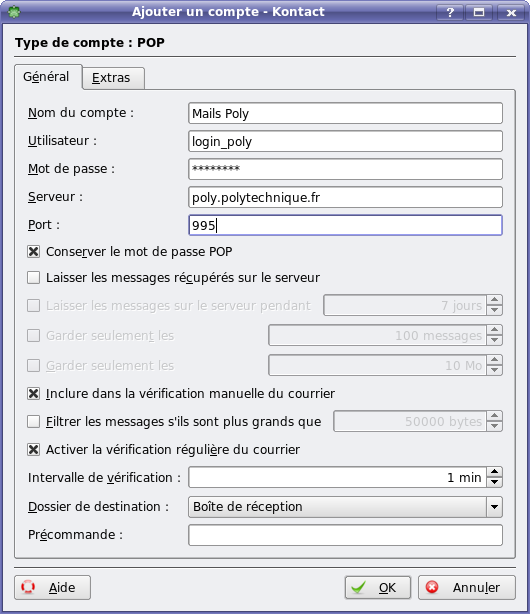
\includegraphics[width=0.48\textwidth]{images/nux_config_kmail_pop} }
      \hspace{\stretch{1}}
      \subfloat[Envoi des messages]{ 
 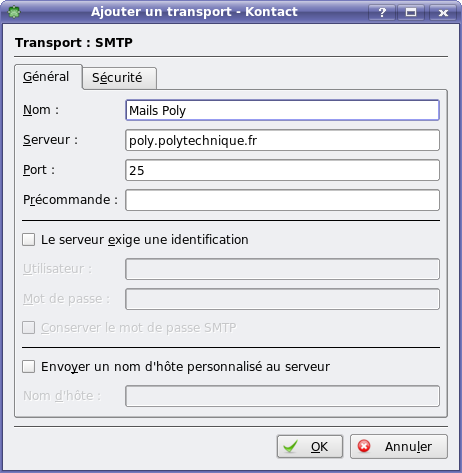
\includegraphics[width=0.48 \textwidth]{images/nux_config_kmail_smtp} }
 \caption{Configuration sous \app{Kmail}}
    \end{center}
  \end{figure*}


Utilise les param\`etres suivants pour configurer l'onglet \menu{G\'en\'eral} :
\begin{description}
  \item[Nom] le nom du compte, par exemple : Mails Poly
  \item[Utilisateur] rentre le \emph{login} \server{poly} que t'a fourni la DSI \`a  ton arriv\'ee sur le plateau
  \item[Mot de passe] et l\`a  le mot de passe \server{poly}
  \item[Serveur] \server{poly.polytechnique.fr}
  \item[Port] 995
\end{description}
Ensuite, va dans l'onglet \menu{Extras} et coche la case
\menu{Utiliser SSL pour s\'ecuriser les t\'el\'echargements}.

Maintenant, dans l'onglet \menu{Envoi des messages} clique sur le
bouton \menu{Ajouter\ldots}. Utilise les param\`etres suivants pour le
configurer :
\begin{description}
  \item[Nom] le m\^eme nom de compte que pr\'ec\'edemment
  \item[Serveur] \server{poly.polytechnique.fr}
  \item[Port] 25
\end{description}
Sinon, laisse toutes les cases d\'ecoch\'ees.

%Tu peux aussi configurer l'acc\`es \`a  \app{l'annuaire LDAP} de l'\'Ecole, sorte de carnet d'adresses en ligne qui contient les adresses \emph{mail} de tout le monde sur le campus. Pour ce faire, commence par ouvrir \menu{Outils}, \menu{Carnet d'adresses}, puis va dans \menu{Configuration}, \menu{Configurer kAdressBook}, \menu{Consultation LDAP}. Clique ensuite sur \menu{Ajouter un h\^ote}, et configure comme suit: \\
%\smallskip
%\begin{minipage}[t]{0.48\textwidth}
%\begin{description}
%  \item[H\^ote] \server{ldap.eleves.polytechnique.fr}
%  \item[Port] 389
%  \item[Version de LDAP] 3
%\end{description}  
%\end{minipage} 
%\begin{minipage}[t]{0.48\textwidth}
%\begin{description}  
%  \item[DN] \server{dc=polytechnique, dc=ldap, dc=eleves, dc=fr}
%  \item[S\'ecurit\'e] Non
%  \item[Identification] Anonyme
%\end{description}
%\end{minipage} \\
%Une fois revenu dans \menu{Configuration LDAP}, coche la case \server{ldap.eleves.polytechnique.fr}. Tu as maintenant acc\`es \`a  l'annuaire LDAP lors de la
%r\'edaction de messages, avec tout au plus un red\'emarrage de \app{Kmail}. 
%
%\imagepos{images/nux_config_ldap}{0.55}{Configuration de l'annuaire LDAP sous Kmail}{pht}
%\imagepos{images/nux_config_knode}{0.45}{Configuration de Knode}{ht}
%
%\noindent
%  \begin{figure*}[!h]
%    \begin{center}  
%      \subfloat[Configuration de l'annuaire LDAP sous Kmail]{ 
%      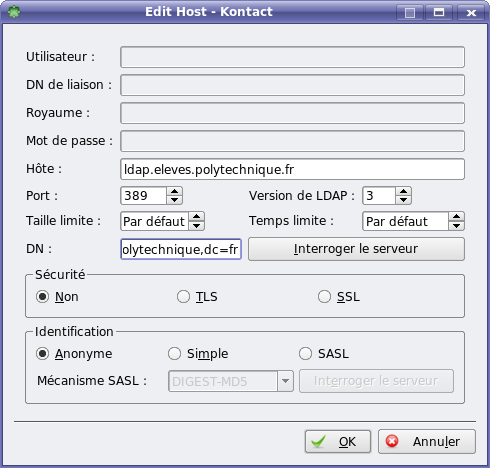
\includegraphics[width=0.48\textwidth]{images/nux_config_ldap}}
%      \hspace{\stretch{1}}
%      \subfloat[Configuration de Knode]{ 
% 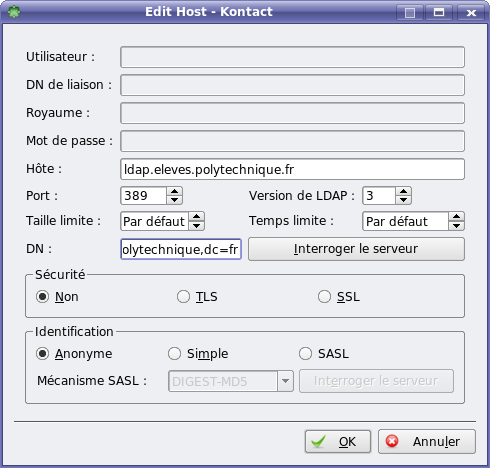
\includegraphics[width=0.48 \textwidth]{images/nux_config_ldap} }
% \caption{Configurations LDAP et \emph{news}}
%    \end{center}
% \end{figure*}


\paragraph{Mac OS Mail}

\flimage{images/mac_mail_icone}{0.07}{l} \app{Mail} : un client \emph{mail} offrant les fonctionnalit\'es classiques d'un bon client : recherche instantan\'ee, filtre antispam, r\`egles de tri automatique des \emph{mails}, regroupement des \emph{mails} correspondant \`a  une m\^eme discussion.

Au premier lancement, \app{Mail} te demandera de remplir les informations concernant ton compte \emph{mail} sur \server{poly}, il suffit de le remplir avec les donn\'ees suivantes :
\begin{description}
  \item[Nom complet] ton nom !
  \item[Adresse \'electronique] de la forme \mail{prenom.nom@polytechnique.edu}
  \item[Serveur de r\'eception] \server{poly.polytechnique.fr}
  \item[Type de compte] \menu{POP}
  \item[Nom d'utilisateur] ton \emph{login} \server{poly} (les huit premi\`eres lettres de ton nom en g\'en\'eral)
  \item[Mot de passe] ton mot de passe \server{poly}
  \item[Serveur d'envoi (SMTP)] \server{poly.polytechnique.fr} ou \server{ssl.polytechnique.org}
\end{description}

Si tu as d\'ej\`a  cr\'e\'e un compte pr\'ec\'edemment, il faut aller dans les \menu{Pr\'ef\'erences} (accessibles depuis le menu \menu{Mail}), onglet \menu{Comptes}, pour cr\'eer un autre compte en cliquant sur la case \menu{+}.

N'oublie pas de cocher \menu{Activer le cryptage SSL} dans l'onglet \menu{Avanc\'e}, port 995. Tu souhaiteras alors certainement installer le certificat de s\'ecurit\'e de \server{poly} (tu le trouveras sur \urllink{http://poly/}). Une fois que tu as t\'el\'echarg\'e le certificat, ouvre le fichier \menu{.CRT} obtenu, et dans \app{Trousseau d'acc\`es}, installe-le dans %\menu{X509Anchors} (Tiger) ou 
\menu{session} (Leopard).

Cette configuration marche pour acc\'eder \`a  ses mails depuis l'int\'erieur de l'X mais aussi de l'ext\'erieur, sans rien changer. En revanche tu ne peux pas envoyer de \emph{mails} depuis l'ext\'erieur , car le serveur \server{poly} ne le permet pas. Nous te conseillons vivement d'utiliser le serveur SMTP \server{polytechnique.org} et de regarder la configuration propos\'ee par \urllink{Polytechnique.org}. Celle-ci permet d'envoyer des \emph{mails} s\^urs \`a  l'ext\'erieur de l'\'Ecole sans modifier ta configuration par la suite. Tu peux ajouter ce SMTP dans l'onglet \menu{Comptes} des \menu{Pr\'ef\'erences} de \emph{mail} et r\'egler dans l'onglet \menu{Avanc\'es} comme dans la capture.

\begin{figure*}[!hl]
    \begin{center}
            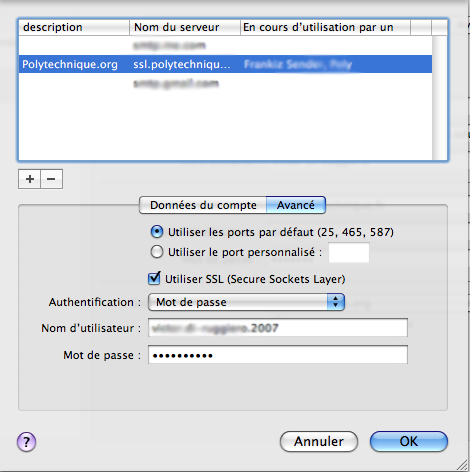
\includegraphics[width=0.4\textwidth]{images/mac_config_smtp_poltechnique.png} 
      \caption{Configurer le serveur SMTP \server{Polytechnique.org}}
    \end{center}
  \end{figure*}

%Le LDAP ne fonctionne pas \`a  l'heure actuelle avec \app{Mail} (mars 2009) sous \app{Leopard}, contrairement aux  autres syst\`emes d'exploitation (fonctionne cependant avec \app{Thunderbird}).
%\subsuEnfin, tu peux disposer dans \app{Mail} de l'annuaire de l'\`acole, mis \`a  disposition par la DSI. Pour cela, va dans les \menu{Pr\'ef\'erences} de Mail,
%puis dans la rubrique \menu{R\'edaction} et clique sur \menu{Configurer LDAP\ldots}. Tu peux ensuite utiliser le bouton \menu{+} pour ajouter un
%serveur, et remplir la fen\^etre comme sur la capture.

%\imagepos{images/mac_config_ldap}{0.6}{Configurer l'annuaire}{!ht}
%bsection{Logiciels additionnels}

%Les logiciels suivants sont utiles pour utiliser avec Mac OS X les services propos\'es sur le r\'eseau ; ils sont t\'el\'echargeables sur \server{frankiz}, dans la rubrique \menu{T\'el\'echarger}, \menu{Mac}.



%%%%%%%%%%%%%%%%%%%%%%%%%%%%%%%%%%%%%%%%%%%%%%%%
% ANCIENNE CONFIGURATION DES BR POUR CHAQUE OS %
%%%%%%%%%%%%%%%%%%%%%%%%%%%%%%%%%%%%%%%%%%%%%%%%

%% VIEILLE PAGE DE CONF NEWSGROUP POUR WINDOWS

%\subsubsection{Configuration \emph{newsgroups}}
%
%Reporte-toi a la page~\pageref{newsgroups} pour la description et des d\'etails de fonctionnement des \emph{newsgroups} \`a  l'X.
%
%Comme pour les \emph{mails}, nous d\'ecrivons la configuration de \app{Outlook Express} mais elle est sensiblement \'equivalente pour \app{Thunderbird}. Lance
%\app{Outlook Express} et va dans le menu \menu{Outils}, \menu{Comptes\ldots}. Clique sur le bouton \menu{Ajouter\ldots} en haut \`a  droite,
%\menu{News\ldots}. Remplis les \'ecrans de configuration suivants avec ces donn\'ees :
%\begin{description}
%  \item[Nom complet] ton nom !
%  \item[Adresse de messagerie] de la forme \mail{prenom.nom@polytechnique.edu}
%  \item[Serveur de news (NNTP)] \server{news} ; v\'erifie \`a  ce moment que la case
%       \menu{Connexion \`a  mon serveur de news requise} n'est pas coch\'ee.
%\end{description}
%Voil\`a , clique sur \menu{Continuer}, \menu{Terminer}; tu es abonn\'e
%au serveur \emph{news} des \'el\`eves.
%
%Quand tu fermeras la fen\^etre `Comptes Internet', il va te demander \`a 
%quels \emph{newsgroups} tu veux t'abonner, tu n'auras qu'\`a  s\'electionner
%ceux qui t'int\'eressent. Reporte-toi \`a  la page \pageref{newsgroups}
%pour plus d'infos sur les newsgroups auxquels t'abonner !
%
%Si tu veux t'inscrire \`a  d'autres serveurs \emph{news}, refais cette
%proc\'edure en rentrant le nom du serveur qui t'int\'eresse \`a  la place
%de \fkz.
%\setcounter{page}{12}

%% VIEILLE PAGE DE CONF NEWSGROUPS POUR LINUX


%\subsubsection{Configuration \emph{news}}
%
%\flimage{images/nux_knode_icon}{0.12}{l} Le client \emph{news} le plus utilis\'e est \app{Knode}. Parmi les autres clients \emph{news}, citons 
%\app{Thunderbird}, \app{Pan} ou \app{slrn}. Ici aussi, la configuration est presque ind\'ependante du logiciel choisi.
%
%
%Sous \app{Knode}, c'est dans le menu \menu{Configuration}, puis \menu{Configurer Knode}. Va dans la rubrique \menu{Comptes, Forums de discussion} et
%cr\'ee un compte en cliquant sur \menu{Ajouter\ldots}.
%
%\imagepos{images/nux_config_knode}{0.45}{Configuration de Knode}{ht}
%
%\pagebreak
%
%Remplis l'onglet \menu{Serveur} avec les informations suivantes :
%\begin{description}
%  \item[Nom] ce que tu veux pour d\'ecrire ce compte, par exemple 'News Frankiz'
%  \item[Serveur] \server{news}
%\nopagebreak  \item[Port] 119
%\end{description}
%
%\pagebreak
% 
%Ensuite occupe-toi de l'onglet \menu{Identit\'e} :
%\begin{description}
%  \item[Nom] mets ton pseudo dans ce champ
%  \item[Organisation] X, \'Ecole polytechnique, comme tu le sens
%  \item[Adresse \'electronique] ton adresse \emph{mail}, pour que les gens puissent te r\'epondre par \emph{mail}.
%\end{description}
%
%Enfin, pour que \app{Knode} puisse envoyer des \emph{mails}, il faut aller
%dans la rubrique \menu{Comptes}, sous-rubrique \menu{Serveur de
%courrier (SMTP)}, et choisir comme serveur d'envoi de \emph{mails}
%\server{poly.polytechnique.fr}, port 25 --- c'est exactement la m\^eme
%configuration SMTP que \app{Kmail}.
%
%Si tu veux mettre une signature \`a  la fin des messages que tu
%posteras, il te suffit de la mettre dans l'onglet \menu{Identit\'e}.
%Sur la plupart des clients la signature est interpr\'et\'ee comme
%ext\'erieure au message et n'est en particulier pas incluse dans le
%texte cit\'e lorsque tu r\'eponds \`a  un message. Pour d\'efinir une
%signature \`a  la main, il suffit de mettre \verb*+-- +\ (c'est \`a  dire
%-{}-<espace>) sur une ligne, et tout ce qui suivra cette ligne
%composera ta signature.
%
%Il ne te reste plus qu'\`a  t'inscrire \`a  des \emph{newsgroups} (reporte-toi \`a  la page \pageref{newsgroups} pour plus d'infos) et \`a  poster ! \\
%
%Pour te connecter aux serveurs de \emph{news} de Polytechnique.org, qui ont un acc\`es s\'ecuris\'e, avec \app{Knode}, il y a une petite subtilit\'e car il
%ne g\`ere pas le SSL. Il faut installer \app{stunnel} qui permet de d\'efinir une redirection SSL de port. Dans \file{/etc/stunnel.conf} (ou parfois \file{/etc/stunnel/stunnel.conf}), mets les lignes suivantes (les trois premi\`eres y sont en principe d\'ej\`a ) :
%\cmdline{\# location of pid file\\
%pid = /etc/stunnel/stunnel.pid\\
%\\
%\# user to run as\\
%setuid = stunnel\\
%setgid = stunnel\\
%\\
%\# Use it for client mode\\
%client = yes\\
%\\
%\# sample service-level configuration\\
%{[}nntps{]}\\
%accept  = 1119\\
%connect = ssl.polytechnique.org:563\\
%TIMEOUTclose = 0
%}
%
%Il ne te reste plus qu'\`a  lancer \app{stunnel} par :
%\cmdline{/etc/init.d/stunnel start}
%
%Et tu peux ainsi lire les \emph{news} de Polytechnique.org en mettant \server{localhost} comme serveur et
%\server{1119} comme port. Il faut aussi que tu coches \menu{Le serveur exige une identification} et
%que tu rentres ton nom d'utilisateur \`a  Polytechnique.org et ton mot de passe, que tu peux d\'efinir
%sur \urllink{https://www.polytechnique.org/Xorg/SMTPSecurise}.

%% VIEILLE PAGE DE CONF NEWSGROUP POUR MAC


%\subsubsection{Configuration \emph{news}}
%
%\flimage{images/mac_thunderbird_icone}{0.07}{l} 
%\app{Thunderbird} : un client \emph{news} permettant d'acc\'eder aux forums de discussion des \'el\`eves (voir page~\pageref{newsgroups} pour les d\'etails sur \server{frankiz}), mais aussi \`a  ceux de \server{usenet} gr\^ace au serveur \server{polynews.polytechnique.fr}. Il est tr\`es proche d'\app{Outlook Express} dans son esprit. Dans la m\^eme cat\'egorie, il existe \app{MacSOUP}, \app{Unison} ou encore \app{MT-NewsWatcher}. La configuration se fait de la m\^eme mani\`ere.
%
%Au premier lancement, l'application te propose d'importer les param\`etres depuis une autre application. Clique sur \menu{Suivant}. Tu peux alors choisir quel type de compte tu veux configurer (tu remarqueras que tu peux aussi cr\'eer un compte courrier \'electronique, et un compte RSS). S\'electionne \menu{Compte forums de discussion} et clique sur \menu{Suivant}. Entre alors les informations suivantes :
%
%\begin{description}
%  \item[Votre nom] ton nom ou ton pseudo
%  \item[Adresse de courrier] \mail{prenom.nom@polytechnique.edu}
%  \item[Serveur de forums] \server{news}
%  \item[Nom du compte] News Frankiz
%  \item[Nom d'utilisateur] ton \emph{login }poly (les huit premi\`eres lettres de ton nom en g\'en\'eral)
%  \item[Serveur d'envoi (SMTP)] \server{poly.polytechnique.fr} ou \server{ssl.polytechnique.org}
%\end{description}
%
%
%Pour t'abonner \`a  des groupes de discussion, il te suffit de s\'electionner le compte \menu{News Frankiz} dans la fen\^etre \menu{Dossiers} de \app{Thunderbird}, puis de cliquer sur \menu{G\'erer les abonnements aux groupes de discussion}. Tu pourras ensuite s\'electionner les forums qui t'int\'eressent parmi la liste propos\'ee. Reporte-toi \`a  la page \pageref{newsgroups} pour plus d'infos sur les \emph{newsgroups} auxquels t'abonner !
%

\label{wifi}
\subsection{\emph{Wi-Fi}}
La DSI propose actuellement un réseau \emph{Wi-Fi}, qui couvre le grand hall, les amphis, les salles de PC, le bataclan (bâtiment qui va de la Kès au bâtiment des
binets/langues), le bâtiment des binets/langues.

Pour te connecter au \emph{Wi-Fi} avec Windows, Mac, Linux ou un iPhone, tu trouveras les instructions sur la page \urllink{http://wifi}.

Avec Windows, \textbf{avant Windows 8}, tu dois téléchager un logiciel appelé \app{SecureW2} qui est fourni par la DSI sur son site, \urllink{http://www.dsi.polytechnique.fr/fr/telecommunications/wifi/}. Ce n'est plus nécessaire depuis Windows 8.

Avec Mac OS X Lion ou iOS (iPhone, iPad), il faut télécharger un fichier 
\newline \file{Ecole-Polytechnique.mobileconfig} dont le lien se trouve sur \urllink{http://wifi}. Pour des versions plus anciennes de Mac OS, consulte \urllink{http://br.binets.fr/Configuration\_du\_WiFi\_sous\_Mac}. Attention, avec iOS7, il arrive que le fichier .mobileconfig fourni par la DSI ne marche pas, tu peux essayer avec celui là: \urllink{br.binets.fr/files/WifiPoly.mobileconfig}.

Avec Linux ou Android, les noms des paramètres dépendent du système utilisé, mais voici un tableau récapitulatif :
\begin{center}
\begin{tabular}{r|l}
 SSID & Polytechnique \\
 Nom d'utilisateur/Mot de passe & Identifiants DSI (salle info) \\
 Sécurité & WPA1 Entreprise \\
 Gestion des clés & WPA-EAP \\
 Pairwise & TKIP \\
 Authentification & Tunneled TLS (TTLS) ou EAP-FAST \\
 Authentification interne & PAP \\
 Proxy HTTP pour tous les protocoles & 129.104.247.2 (port 8080) \\
 Serveurs DNS & 129.104.201.53, 129.104.201.51
\end{tabular}
\end{center}




%Deux réseaux ont été déployés :

%\begin{description}
%  \item[keriadenn] : c'est le réseau public, qui te permet uniquement d'accéder au portail wifi (\url{http://wifi/}, accessible également depuis le réseau normal). Tu trouveras à cette adresse toutes les informations de configuration nécessaires pour te connecter au second réseau, \server{kastell}.

%  \item[kastell] : réseau protégé et caché qui permet, après authentification, de te connecter au réseau et à Internet comme si tu étais dans ton casert !
%\end{description}


% -------------------- Puis... --------------------
%\setlength{\parskip}{7pt}
\bghdr{images/fond-infobr}
\markright{Pour continuer}
%$Id: partie2.tex 110 2005-03-02 15:56:44Z myk $
\clearpage
\section{Présentation du réseau et de plusieurs services}
\label{services}


\subsection{Une source d'informations inestimable : le WikiX}
\label{WikiX}
Bien que n'étant pas à proprement parler un service du Binet Réseau, un site un peu particulier connu sous le nom de \textbf{WikiX} est hébérgé sur un des serveurs du BR.
C'est un wiki qui rassemble toutes les informations dont tu peux avoir besoin sur le plâtal.
Le plus court moyen d'y aller est de taper \urllink{wikix} dans la barre d'adresse de ton navigateur, mais il y a aussi un lien vers le WikiX sur \fkz dans le menu navigation.

La première fois que tu te connectes sur le WikiX il faut que tu t'identifies (identification \emph{via} \urllink{polytechnique.org});
ensuite ton navigateur gardera un cookie qui t'identifiera à chaque connection si tu le souhaites. \emph{Tu ne peux lire et modifier le WikiX que si tu es identifié !}

Tu es bien entendu encouragé à contribuer au WikiX pour faire profiter les autres de ton expérience, 
soit en modifiant ou en mettant à jour un article existant, soit en créant un nouvel article qui manquait au WikiX.


Tu te rendras vite compte que \emph{peu importe l'information que tu cherches, elle est sur le WikiX.}

\subsection{Polytechnique.org}
\urllink{Polytechnique.org} est une association loi 1901 compos�e d'�l�ves et d'Anciens �l�ves
 ind�pendante de l'administration de l'�cole (et donc des domaines \server{polytechnique.fr}
 et \server{polytechnique.edu}).

Le but de l'association est la mise � disposition des X d'outils
ayant un rapport avec l'Internet, entre autres :
\begin{itemize}
  \item des redirections mails nombreuses (adresses suppl�mentaires) et � vie ;
  \item un serveur de news (comme les br.*), ouvert aux Anciens et aux non-plat�liens ;
  \item une facilitation des contacts vers les Anciens et les camarades de promotion ;
  \item une lettre mensuelle, pour s'informer sur l'actualit� de la communaut� polytechnicienne ;
  \item des annonces d'�v�nements ;
  \item des services d'h�bergement pour les groupes et binets, notemment des noms de domaine (via \server{www.po\-ly\-tech\-ni\-que.net}) et des listes de diffusion (\mail{br2005@po\-ly\-tech\-ni\-que.org}, par exemple).
\end{itemize}
Si tu veux d�couvrir les autres services de l'association ou savoir
comment les utiliser, tu peux aller sur la page
\urllink{https://www.polytechnique.org/Xorg/Xorg} (accessible depuis
le lien Documentations dans le menu de \urllink{Po\-ly\-tech\-ni\-que.org}
quand tu est connect�).

Par ailleurs, les filtres antivirus et antispam appliqu�s � sur les mails sont tr�s efficaces (99\% de rep�rage correct), et polytechnique.org te conseille donc de mettre en place la redirection suivante :
\mail{prenom.nom@polytechnique.edu}
redirig�e sur \mail{prenom.nom(.promo)@po\-ly\-tech\-ni\-que.org},
elle-m�me redirig�e vers \mail{login@poly(.po\-ly\-tech\-ni\-que.fr)}.
Pour effectuer ces redirections, connecte-toi sur les pages suivantes :
\begin{itemize}
  \item pour \mail{@polytechnique.edu} : \urllink{https://www.mail.polytechnique.edu} ;
  \item pour \mail{@polytechnique.org} : \urllink{https://www.polytechnique.org} ;
  \item pour \mail{@poly} : \urllink{http://poly.polytechnique.fr}.
\end{itemize}
Cela est expliqu� plus en d�tails sur la page
\urllink{https://www.polytechnique.org/Xorg/Re\-di\-rec\-tion\-Mails}.

Ces outils sont tr�s utiles, et faciles � s'approprier, que
ce soit pour toi, pour tes binets, ou pour (dans le
futur) garder contact avec la communaut� polytechnicienne. Rejoins
les 15000 camarades d�j� inscrits !

En cas de probl�me, n'h�site pas � contacter
\mail{contact@polytechnique.org}.


\subsection{Partager tes fichiers sur le r\'eseau avec FTP}
\bghdr{images/fond-infobr}

Les \'echanges de fichiers sur le r\'eseau \'el\`eves se font souvent par FTP. Rien de plus simple que de partager toi aussi tes pr\'ecieuses donn\'ees en installant un serveur FTP !

\paragraph{Client FTP}
Pour une utilisation basique, taper \urllink{ftp://nom-du-ftp}  (par exemple \urllink{ftp://jtx} dans la barre d'adresse de ton navigateur suffit \`a parcourir les fichiers propos\'es par \og Gentil Vieux-Chouffe \fg.
Pour une meilleure utilisation, le BR te conseille \app{FileZilla}. T\'el\'echarge-le sur \urllink{http://www.filezilla.fr} et double-clique sur l'installeur.
Tu pourras d\`es la fin de l'installation aller sur tous les FTP du r\'eseau facilement et rapidement.\\
\flimage{images/mac_cyberduck_icone}{0.07}{l} \app{Cyberduck} est un autre client FTP tr\`es simple \`a  utiliser mais performant. Il te permettra d'aller t\'el\'echarger des fichiers sur les serveurs FTP des autres \'el\`eves sans probl\`eme.\\
Pour se connecter \`a  un serveur, il suffit de taper son nom (exemple : \urllink{jtx}) dans le cadre \menu{Connexion rapide} puis d'appuyer sur Entr\'ee.\\


\paragraph{Serveur FTP}
Tu verras rapidement que tout le monde \`a  l'X poss\`ede un serveur FTP
afin de partager les diff\'erents projets, les films du JTX, ses
photos, etc. Il est donc quasiment indispensable que tu en installes un.\\

Parmi les plus simples on trouve \app{FileZilla Server} et \app{GuildFTP}, qui sont libres de surcro\^{i}t.
Si tu es sous mac, tu peux aussi jeter un \oe{}il à \app{PureFTPd Manager}, qui est très pratique à utiliser.\\
Quoiqu'il en soit, tu trouveras toutes les informations n\'ecessaires \`a la configuration de ton serveur FTP sur \urllink{http://wikix.polytechnique.org/FTP}.\\
Pense \`a lui donner un nom sur \urllink{http://dnsapp/} (voir aussi page \pageref{dnsapp})


\subsection{Avoir un nom sur le r\'eseau}


\subsection{Services propos\'es aux binets}

Le BR propose plusieurs services aux binets :
\begin{itemize}
\item une adresse \emph{mail} en \mail{nom\_du\_binet@binets.polytechnique.fr} qui permet de contacter les administrateurs \fkz\ du binet ;
\item le référencement des membres grâce au TOL ;
\item des annonces (une seule visible par binet) sur \fkz\ quand le binet veut faire de la pub ;
\item les Platalpads de binet (\urllink{http://nom\_du\_binet.platalpad}), accessibles aux membres du groupe \fkz\ (voir p. \pageref{platalpad}).
On s'y connecte en utilisant ses identifiants \fkz. Ce service fonctionne aussi \`a l'ext\'erieur via
\urllink{https://www.polytechnique.fr/eleves/platalpad/nom\_du\_binet}.
\end{itemize}

Pour disposer de ces services, il te suffit de remplir les fiches qui sont dans la case du BR à la Kès. Il faut à la création et à la passation du binet
donner au BR les noms du prez et du webmestre de ton binet ainsi que, si tu désires que ton site soit accessible à l'extérieur, une fiche pour la DSI et nous.

Le BR propose également aux binets qui le souhaite d'héberger leur site Internet. Ce site peut être interne (visible uniquement depuis l'X) ou externe (visible de l'extérieur de l'X).
Les sites binets disposent de PHP et MySQL, et bénéficient d'une capacité de stockage (extensible) de 100 Mo.

Les sites ayant une visibilité extérieure doivent satisfaire aux conditions suivantes :
\begin{itemize}
    \item Aucune information ne doit être diffusée qui pourrait nuire à l'image de l’École. (photos, vidéos, etc.) En particulier son contenu doit respecter la loi française sur les droits d'auteur.
    \item Le site doit avoir une qualité visuelle, si ce n'est professionnelle, du moins très correcte.
    \item Le site ne doit pas héberger de vidéos ou diffuser un flux vidéo (streaming). Toutes les vidéos du sites doivent être hébergées à l'extérieur. (Dalymotion, YouTube, etc.)
    \item Les images présentes sur le site ne doivent avoir une résolution suffisamment faible afin de ne pas saturer la bande passante vers l'extérieur. 
\end{itemize}

Le BR offre ce service gratuitement, en partie grâce à une subvention de la Kès.
Il se réserve le droit de refuser ou d'interrompre l'hébergement d'un site, sans préavis, sans recours possible et sans avoir à fournir de motif.
Il s'engage à en informer immédiatement le bureau du binet concerné. 

\subsection{Un outil de travail collaboratif : Platalpad}
\label{platalpad}

Platalpad est un éditeur de texte collaboratif par navigateur, un peu comme un google doc. Il permet de travailler à plusieurs sur un même document, chacun voyant les modification des autres. Il est donc très pratique pour s'organiser.\\
Il se décline en deux versions :
\begin{itemize}

\item \textbf{Platalpad généraliste :} rends-toi tout simplement sur \urllink{http://platalpad/} pour créer un nouveau document. Ensuite, il suffit de diffuser son adresse à toutes les personnes que tu veux voir prendre part à sa réalisation. \\

\item \textbf{Platalpad privé :} Chaque binet se voit automatiquement, une fois inscrit sur \fkz, attribué un espace privé, accessible seulement à ses membres. Tu peux y accéder à partir de la page \fkz du binet en question ou directement sur \urllink{http://nom-du-binet.platalpad/}. Une fois identifié, tu peux voir chacun des documents en cours de réalisation au sein du binet et les modifier à ta guise.

On s'y connecte en utilisant ses identifiants \fkz. Ce service fonctionne aussi à l'extérieur via : 
\urllink{https://www.polytechnique.fr/eleves/platalpad/nom\_du\_binet} ;

\end{itemize}

\imagepos{images/platalpad}{0.7}{Un document en cours d'édition sur un platalpad privé}{!h}

%$Id: irc.tex 144 2005-03-25 01:11:37Z myk $

\subsubsection{IRC}

\label{irc}

%IRC est un autre moyen de communication mis à ta disposition par le Binet Réseau. Il s'agit d'un système de \emph{chat} (messagerie instantanée) permettant à la fois de dialoguer à plusieurs dans des \emph{salons}, mais également d'avoir des conversations privées avec d'autres personnes connectées.

IRC is a communication device provided by the Binet Reseau. It is a \emph{chat} software
enabling a multi-user conversation within \emph{channels}, as well as private chats with other connected people.

The Binet Reseau's IRC server is connected to RezoSup, an IRC network gathering lost of french engineering schools and universities.

%Le serveur IRC du Binet Réseau est relié à RezoSup, réseau IRC des grandes écoles d'ingénieurs et université française.

%Pour te connecter sur IRC tu disposes de deux méthodes:
There are two ways for you to connect to IRC :


\begin{description}
  \item[using an IRC client:] we recommend the use of \app{X-Chat} (available in the \emph{Télécharger} part on  \fkz). Use \server{ircserver} as server, and \server{6667} (default port) as port.
  \item[using the web interface:] go to \urllink{http://ircserver/}, or follow the link \menu{Accéder à IRC} on \fkz. Thus you'll be able to use the IRC without installing anything.
 \end{description}

Here are some channels you might find usefull :
 \begin{itemize}

  \item \ngname{\#x} the channel for all students at the Ecole Polytechnique.
  \item \ngname{\#linux} if ever you have questions about linux
  \item \ngname{\#superquizz} an online quizz(type \texttt{!nick x} when login in)
  \item \ngname{\#br} the Binet Reseau's channel
 \end{itemize}


%
\subsubsection{Le site du BR : un Wiki}
\label{siteBR}

Le site public du Binet R�seau est disponible sur \url{http://frankiz/binets/reseau/}. C'est un wiki, ce qui permet aux BR-men de le mettre ais�ment
� jour avec les derni�res informations de configuration.

Tu y trouveras un grand nombre d'informations � jour sur le BR, sur les services que nous offrons, et sur nos projets.

Il est compl�mentaire � la {\sc FAQ} et � cet InfoBR : il contient
des informations de configuration pour les services offerts par le
BR et des d�tails pour les projets que le BR m�ne.


%%$Id: qrezix.tex 144 2005-03-25 01:11:37Z myk $

\subsection{La t\'el\'evision du BR}
\label{TV}

Le BR diffuse sur le r\'eseau plusieurs dizaines de chaines de t\'el\'evision et radios. Pour les recevoir, nous recommandons \app{vlc}, disponible sur le X-Share.

\subsubsection{Configuration de vlc}

La liste des cha\^ines est diffus\'ee sous forme d'annonces SAP. Pour voir ces annonces, ouvre ta liste de lecture (Vue -> Liste de lecture), et active la d\'ecouverte de services (\ref{vlc:config}).
Attention sous \app{Windows Vista} un probl\`eme de compatibilit\'e connu entra\^ine un \'ecran noir. Pour le r\'esoudre le BR t'a pr\'epar\'e une page sur le Wikix.

\imagepos{images/vlc_config_sap.png}{0.75}{Configuration de vlc pour la t\'el\'evision par le r\'eseau}{h!}\label{vlc:config}

Tu auras ainsi dans ta liste de lecture les diff\'erents cha\^{i}nes disponibles.

\subsubsection{Autre m\'ethode}

Si ton client pr\'ef\'er\'e ne supporte pas les annonces SAP, ou que les annonces SAP ne marchent pas chez toi, tu peux r\'ecup\'erer la liste des cha\^ines par
PodCast, à l'adresse \url{http://tv.eleves.polytechnique.fr/tvbr.xml}. Sous \app{vlc}, active la d\'ecouverte des services PodCast dans la liste de
lecture (G\'erer > D\'ecouverte de services > Podcast), puis va dans Param\`etres > Pr\'ef\'erences > Liste de Lecture > D\'ecouverte de services > Podcast et
met l'adresse \url{http://tv.eleves.polytechnique.fr/tvbr.xml} dans le champ \guillemotleft~Liste des URLs~\guillemotright .

\subsubsection{Et si ça ne marche toujours pas?}

V\'erifie que tu utilises bien la derni\`ere version de \app{vlc}. Les versions inf\'erieures à 0.8.5 sont connues pour ne pas fonctionner.

Si rien ne marche, la raison la plus probable est un \emph{firewall} qui intercepte les flux t\'el\'es. Configure ton \emph{firewall} afin d'autoriser
ces flux. Sous Linux, les r\`egles \emph{iptables} suivantes suffisent:

  \cmdline[0.85] {
   -A INPUT -i eth0 -d 224.0.0.0/24 -j ACCEPT
   -A INPUT -i eth0 -d 239.255.42.0/24 -s 192.168.225.0/24 -p udp -m udp --dport 1234 -j ACCEPT
   -A INPUT -i eth0 -d 239.255.255.255/32 -p udp -m udp --dport 9875 -j ACCEPT
   -A OUTPUT -o eth0 -d 224.0.0.0/4 -j ACCEPT.
  }


\subsection{Installer et mettre à jour Windows ou Linux}

\subsubsection{Licences de produits Microsoft}
\label{msdnaa} Les accords n\'egoci\'es par le BR avec Microsoft dans le cadre de MSDNAA donnent \`a  chaque X le droit de poss\'eder une version de Windows
XP Pro, de Windows Vista Business ou de Windows 7 Pro gratuite et l\'egale, ainsi que les licences pour la plupart des logiciels de la soci\'et\'e (quasiment tous, sauf
Office et les jeux). La seule condition \`a  remplir est d'\^etre \'etudiant sur le pl\^atal au moment de l'installation du logiciel ; tu pourras ensuite le
garder sur ton PC m\^eme apr\`es ton d\'epart de l'X.

La proc\'edure pour obtenir les logiciels et les cl\'es correspondantes
est la suivante :
\begin{itemize}

\item Va d'abord sur \fkz et connecte-toi, puis clique sur le lien \menu{Licences MSDNAA} qui se trouve dans la rubrique \menu{Administration}. S\'electionne le logiciel que tu souhaites installer et valide ta demande, tu recevras ta cl\'e par e-mail. Facile ! Si jamais le logiciel n'est pas dans la liste propos\'ee, c'est soit qu'il n'y a pas besoin de cl\'e --- c'est le cas de beaucoup des logiciels autres que Windows, soit qu'on a oubli\'e de l'y mettre ; dans ce cas, \'ecris \`a  \mail{msdnaa@eleves} pour qu'on t'attribue manuellement une cl\'e.

\item Maintenant que tu as ta cl\'e, il faut t\'el\'echarger le logiciel proprement
dit. Pour cela, connecte-toi par FTP sur \urllink{ftp://miroir/windows/msdnaa/} avec ton client FTP pr\'ef\'er\'e. Tu pourras, selon le logiciel, y r\'ecup\'erer soit une image du CD de type \file{logiciel.iso} (\`a 
graver ou \`a  utiliser avec \app{Daemon Tools}), soit directement le contenu du CD.
 
\end{itemize}

\subsubsection{Miroirs GNU/Linux}

Le BR propose sur \urllink{ftp://miroir/} des miroirs de plusieurs distributions GNU/Linux. Leur avantage principal est que le téléchargement se fait directement sur le réseau local, donc \emph{très} rapidement.
Les miroirs suivants sont disponibles:

\begin{itemize}
\item \distrib{Cygwin} (Environnement Unix pour Windows);
\item \distrib{Debian} (CDs, distribution et mises à jour);
\item \distrib{Gentoo} (CDs, distribution et mises à jour);
\item \distrib{Ubuntu} (CDs, distribution et mises à jour);
\item \distrib{Fink} (Nombreux logiciels Unix/Linux adaptés pour Mac OS).
\end{itemize}

Les miroirs évoluent régulièrement. Tu peux te référer \`a la page \pageref{ubuntu_mirror} pour leur configuration sous \distrib{Ubuntu} ;
pour les autres, toutes les informations pour leur utilisation sont disponibles sur \urllink{https://br.binets.fr/Miroir\_FTP}.

%Pour Windows, les fichiers ISO \`a  t\'el\'echarger sont les suivants :
%\begin{description}
%\item[Pour Windows XP]
%\urllink{ftp://miroir/windows/msdnaa/Windows\%20XP/Francais/fr\_windows\_xp\_professional\_with\_service\_pack\_3\_x86\_cd\_x14-80440.iso}.
%
%\item[Pour Windows Vista]
%L\`a , il y a deux possibilit\'es :
%\begin{description}
%\item[Si tu as un processeur 64 bits :] L'image \`a  t\'el\'echarger est dans\\
%\urllink{ftp://miroir/msdnaa/win\_vista\_business\_avec\_sp1/dvd\_64bits/francais/}. Attention, cette
%image ISO est \`a  graver sur un DVD. On remarque aussi que parfois, m\^eme sur un processeur 64 bits il
%vaut mieux choisir la version 32 bits de Windows (celle qui est dans le prochain \emph{item}) pour des
%raisons de disponibilit\'e de pilotes.
%\item[Si tu as un processeur 32 bits :] L\`a , tu peux choisir de graver :
%\begin{itemize}
%\item soit un DVD, dans \\
%\urllink{ftp://miroir/msdnaa/win\_vista\_business\_avec\_sp1/dvd\_32bits/francais/};
%\item soit quatre CDs, que tu trouveras dans \\
%\urllink{ftp://miroir/msdnaa/win\_vista (version CD)/cd\_32bits/french/}.
%
%\end{itemize}
%\end{description}
%
%\item[Pour Windows 7]
%Comme pour Vista, deux possibilit\'es selon ton processeur. Attention, les images sont \`a graver sur DVD :
%\begin{description}
%\item[Si tu as un processeur 64 bits :] L'image \`a  t\'el\'echarger est dans\\
%\urllink{ftp://miroir/msdnaa/win\_7/french/64 bits/}.
%\item[Si tu as un processeur 32 bits :] L'image \`a  t\'el\'echarger est dans\\
%\urllink{ftp://miroir/msdnaa/win\_7/french/32 bits/}.
%
%\end{description}
%\end{description}
%
%Les versions anglophones de Windows XP, Vista et 7 sont \'egalement disponibles sur \server{miroir}.
%Ainsi, si tu as achet\'e un ordinateur sans OS (et ainsi \'economis\'e environ 150 \euro), tu vas chez un copain, fais les demandes et graves le CD chez lui. Si tu as encore des questions, plus de d\'etails sont donn\'es dans le Wikix et le WikiBR de \fkz.
%



%\subsection{Descriptions des différents serveurs}
{\bf Serveurs du BR :} Voici la liste des serveurs du BR que tu vas
utiliser le plus durant tes deux années sur le platâl, ainsi que
leurs adresses IP et les services qu'ils hébergent. Note que ces services
peuvent à tout moment migrer d'une machine à une autre en cas de
besoin.


\begin{description}
        \item[frankiz] (\server{129.104.201.51}) : DNS secondaire,
        \emph{news}, portail des élèves, sites des binets
        \item[gwennoz] (\server{129.104.201.52}) : DNS secondaire,
        développement, miroirs FTP
        \item[heol] (\server{129.104.201.53}) : DNS principale,
        serveur \app{xNet} (pour \app{qRezix}, voir page~\pageref{qrezix}), serveur IRC
        \item[skinwel] (\server{129.104.201.54}) : DNS secondaire,
        dépôt SVN, télévision
	\item[pellwel] (\server{129.104.201.57}) : télévision
    \item[enez] (\server{129.104.201.61}) : Domaine windows, MSDNAA (logiciels Microsoft gratuits)
\end {description}

{\bf Serveurs de la DSI : } \'Etant donné que le réseau élèves est un
sous-réseau de celui de la DSI, nous utilisons également les
serveurs de celle-ci et les services qu'ils hébergent.

\begin{description}
        \item[kuzh] (\server{129.104.247.2}) : \emph{proxy} http (pour l'Internet), \emph{proxy} ssh pour sortir du plateau, futur \emph{proxy} ftp
        %\item[sil] (\server{129.104.247.3}) : ancien \emph{proxy} ssh double sens et \emph{proxy} ftp en sursis, il est conservé tant qu'il survit, et ne sera pas réparé s'il a des problèmes.
        \item[poly] (\server{129.104.247.5}) : \emph{mails} (réception, envoi), tu trouveras en t'y connectant en http (\urllink{http://poly/}) le certificat de sécurité pour l'authentification sécurisée.
        \item[moned] : serveur d'authentification, permettant de
        changer ton mot de passe \server{moned}. Ce mot de passe est celui qui
        te permet de te connecter et d'utiliser n'importe
        quelle machine de salle info. Ton travail n'étant pas stocké
        en local, il t'est donc accessible quel que soit le PC des salles info depuis
        lequel tu te connectes.
    \item[milou] : serveur NTP (\server{ntp.polytechnique.fr})
\end {description}

\fbox{
\begin{minipage}{0.9\textwidth}
  \bf ATTENTION : Les serveurs de la DSI sont à ta disposition pour
  des usages bien précis et ne servent pas de serveurs de
  stockage. La DSI est assez vigilante
  et elle a pour habitude de sanctionner les abus; cela peut inclure la perte de tes comptes
  \server{poly}, \server{moned} ou \server{sil}.
\end{minipage}
}


\newpage


%$Id: partie2.tex 110 2005-03-02 15:56:44Z myk $

\section{R�f�rence Rapide}

\subsection{Polytechnique.org}
\url{Polytechnique.org} est une association loi 1901 compos�e
d'�l�ves et d'anciens �l�ves
 ind�pendante de l'administration de l'�cole (et donc des domaines \server{polytechnique.fr}
 et \server{polytechnique.edu}).

Le but de l'association est la mise � disposition des X d'outils
ayant un rapport avec l'Internet. En particulier, parmi ces outils
il y a :
\begin{itemize}
  \item des redirections mails nombreuses (adresses suppl�mentaires) et � vie ;
  \item des services de news comme le binet r�seau, mais ouverts aux anciens, et aux non plat�liens ;
  \item des contacts ais�s vers les anciens, les camarades de promotion ;
  \item une lettre mensuelle, pour publier des informations qui toucheront tous les polytechniciens ;
  \item des annonces d'�v�nements ;
  \item des services d'h�bergement pour les groupes et binets, des noms de domaine (via \server{www.po\-ly\-tech\-ni\-que.net}) ;
  \item des listes de diffusion de mails (\mail{br2005@polytechnique.org}, par exemple).
\end{itemize}

Par ailleurs, les filtres antivirus et antispams de polytechnique.org �tant assez efficaces, nous te conseillons de mettre en place la redirection
suivante : adresse \mail{prenom.nom@polytechnique.edu} redirig�e sur l'adresse \mail{prenom.nom(.promo)@polytechnique.org}, elle-m�me redirig�e vers
l'adresse \mail{login@poly(.polytechnique.fr)}. Pour effectuer ces redirections, connecte-toi sur les pages suivantes :
\begin{itemize}
  \item pour l'adresse \mail{@polytechnique.edu} : \url{https://www.mail.polytechnique.edu/} ;
  \item pour l'adresse \mail{@polytechnique.org} : \url{http://www.polytechnique.org} (elle est dr�le celle-l�, hein ?) ;
  \item pour l'adresse \mail{@poly} : \url{http://poly.polytechnique.fr}.
\end{itemize}

Tu remarqueras tr�s rapidement que ces outils sont tr�s utiles, que
ce soit pour toi personnellement ou pour tes binets et pour, dans le
futur, garder contact avec la communaut� polytechnicienne: rejoins
les 13000 camarades d�j� inscrits !


%$Id: questions_reponses.tex 144 2005-03-25 01:11:37Z myk $

\subsection{Questions-réponses}

Les questions les plus courantes sont répertoriées ici pour te faire gagner du temps !

\begin{description}

\item[J'ai une question sur l'informatique] je cherche sur le WikiBR et/ou demande \`a un BRman.

%\item[J'ai perdu mon mot de passe qRezix] je le re-définis dans \menu{Administration / Compte / Mes données réseau} sur \fkz ou directement sur \urllink{http://xnetserver}.

\item[Je veux voir mon pseudo quand j'ai voté à la QDJ] je définis mon pseudo sur ma fiche \linebreak trombino sur la page \menu{Administration / Compte / Profil} sur \fkz.

\item[J'ai un deuxième ordinateur, qu'est-ce que je fais ?] je demande une deuxième adresse IP en envoyant un mail à \mail{root@eleves.polytechnique.fr} en préfixant le sujet par [IP] 

\item[Je n'ai plus de réseau] je vais voir la 4\ieme de couverture.

\item[Je viens de changer de casert/section, il faudrait mettre à jour ma fiche TOL] j'envoie \linebreak un mail à \mail{tol@frankiz} avec les modifications à effectuer ainsi que la raison de ces
modifications.

\item[Mon client mail dit que \guillemotleft~l'autorité de certification est inconnue~\guillemotright ] je vais télécharger le certificat de sécurité sur \urllink{https://poly/} et je l'installe.

\item[Je ne reçois pas mes mails] je vérifie ma redirection sur \urllink{http://poly}.

\item[Si la boite mail poly est saturée] Je me connecte sur :\\
\urllink{https://webmail.enseignement.polytechnique.fr/imp/login.php}, 
login : nom de famille --
password : mdp enex ; et je supprime mes mails.


\item[Je n'arrive pas à me connecter à \server{poly}] j'essaye \server{poly.polytechnique.fr}.

\item[Mon ordinateur n'a pas de nom sur le réseau] je lui en donne un gr\^ace \`a \urllink{http://dnsapp/} .

\item[Je cherche des informations sur l'Ecole] je regarde sur \urllink{http://intranet}.

\item[Je cherche à joindre une personne de l'administration] l'annuaire de l'École est sur \linebreak{} \urllink{http://annuaire/}.

\item[Je cherche le numéro de portable d'un X] \urllink{http://www.polytechnique.org}.

\item[J'aimerais être un geek moi aussi !] j'apprends par c\oe ur \urllink{9gag.com/}.

\end{description}


\subsection{Membres \'eminents du Binet R\'eseau}

Chaque BR-man signale quels syst\`emes d'exploitation il conna\^it.

\mbr{Sigma}{71 66}{\wins \nuxs}{Prez, root, news, devel qrezix, support@windows, support@linux}{Touche à tout, il essaie de suivre tout ce qui se passe (même s'il subit parfois ce qui se passe sur les machines). Il a découvert les Virtualbox et s'amuse à les multiplier. Il se charge de la permanence BR matinale (dès 5-6 heures du matin !)}

\mbr{Nathaniel}{76 83}{\nuxs \wins}{Trez, root, web, tol, news, IRCop, devel@frankiz}{Tyran bisounours des news. Si tu as une question concernant le BR (sauf le support), appelle le, y a de grandes chances que ça le concerne. Sa vie a changé depuis qu'il a découvert la puissance du ssh (puis, plus tard, la puissance du -Y).}

\mbr{J-Philippe}{76 42}{\nuxs}{root, web, tol, news, InfoBR, support@linux, support@\LaTeX{}}{Passionné de typographie et de \LaTeX{}, il était logique que ce soit lui qui s'occupe de l'InfoBR. Ne parle surtout pas de majuscule devant lui, il te prendrait la tête pendant 2 heures pour t'expliquer la différence avec la capitale. \`A part ça, il essayera toujours de trouver un peu de temps pour t'aider si tu as un problème en linux (c'est pas le meilleur) ou en \LaTeX{} (c'est le meilleur!).}

\mbr{simon}{73 75}{\nuxs}{root, IRCop, bll}{Depuis assez peu de temps sous linux, il essaie d'en maîtriser les arcanes les plus t\'en\'ebreuses. Toujours à la rue, mais à un degr\'e variable selon l'heure et le jour.}

\mbr{Totor}{71 96}{\macs}{root, web, tol, news, support@mac, Xshare@mac}{Toujours prêt à aider les macqueux, même en plein milieu de la nuit, et les autres aussi même si il ne comprend pas leur problèmes. Tu le trouveras à coup sûr entre entre son kazert et le BôB dès la fin des cours. Pour les macs addicts, ils trouveront leur bonheur et tous les petits programmes qui vont bien sur son ftp.}

\mbr{Andrei}{76 98}{}{devel@root, devel@frankiz}{}

\mbr{Kithyane}{76 22}{\nuxs \wins}{web, tol, news, BRwoman, devel@frankiz}{Elle a découvert son côté geek en entrant au BR, est passée sous Linux depuis, et s'émerveille des nouvelles possibilités qui s'offrent à elle. Extension spirituelle de Nathaniel pour les validations sur Frankiz et la modération des br, en un peu moins bisounours, peut-être, mais avec le sourire de la BRWoman en plus !}

\mbr{Mikado}{70 90}{\wins}{admin@windows}{Problème avec Windows ou les licences Microsoft ? C'est pour lui!}

\mbr{Jiherr}{72 60}{\macs}{support@mac, respo mac, relex}{}

\mbr{RogerTroutman}{77 00}{\wins}{root, admin@windows, support@windows}{}

\mbr{Boris}{73 70}{\nuxs}{root, devel@qrezix}{Gentooiste, il a choisi la voie de la concaténation des Saints Manuels. Il a abandonné son humanité depuis peu pour devenir une page de manuel à  part entière. Tapez `\texttt{/}' pour rechercher.  }

\mbr{Bruno}{71 29}{\nuxs}{support@linux}{N'hésite pas à m'appeler si tu as un problème avec Linux ou le réseau.}

\mbr{Pom}{77 12}{\wins \nuxs}{web, tol, support@windows, support@linux, support@\LaTeX{}}{Coucou ! Moi c'est Pom (ah mince c'est marqué à gauche... bon ben
sinon, c'est Thomas, ça c'est une info exclusive !). Je suis toujours
prêt à t'aider si tu as le moindre problème ou la moindre question.
Mon but c'est rendre service, donc n'hésite pas ! Ma porte est
toujours ouverte (certes elle est perdue au milieu du 3ème étage de
Maunoury, mais quand même). Je sais comment fonctionne Windows :
clic gauche sur le menu démarrer, puis encore un clic au bon
endroit, et ... Quant à linux, et bien je sais que si je tape
"firefox" j'arrive sur internet ! C'est déjà ça. Sinon je m'y connais
en latex, enfin \LaTeX{} hein! Pas de mauvaise compréhension ;) et je
suis chargé de valider tes annonces frankiz, c'est toujours bon à
savoir ! Bisous !}

\mbr{Ninja}{70 70}{\nuxs}{devel@root, BLL, support@linux}{}

\mbr{Shuba}{71 32}{\nuxs}{devel@root}{}

\mbr{fulanor}{72 56}{\macs}{news}{}

\mbr{Buu-Minh}{72 17}{\nuxs \wins}{devel@root, support@windows, support@linux}{Même si ça ne se voit pas, il sera toujours prêt à t'aider si tu rencontres un problème avec ta machine.}


\subsubsection*{Description rapide des postes}

\begin{description}

  \item[Prez]{(\mail{prez@frankiz}) Poste fictif, qui permet toutefois d'avoir
des relations bien plac\'ees.}

  \item[Trez]{(\mail{trez@frankiz}) Escroc qui cherche uniquement \`a remplir le compte en banque pour organiser un voyage de geeks \`a Redmond, ou plut\^ot Cupertino\dots}

  \item[relex]{Assistant du prez pour les relations avec les \emph{gens}.}

  \item[root]{(\mail{root@frankiz}) Les roots sont les administrateurs du r\'eseau. Ce sont eux qui s'\'evertuent \`a maintenir en \'etat de marche les serveurs, \`a rajouter de nouveaux services et \`a rep\'erer les boulets qui font de la merde sur le r\'eseau. S'il s'agit de g\'erer un compte de binet, utilise plut\^ot \mail{binets@frankiz}.}

  \item[admin@windows] {(\mail{windows@frankiz}) Administrateurs du domaine Windows. En cas de probl\`eme avec Windows, en particulier avec l'antivirus, ce sont les mieux plac\'es pour t'aider ; bien s\^ur c'est plus facile si tu es sur le domaine !
}
  \item[support@windows] {(\mail{support@frankiz}) SOS d\'epannage windows, j'\'ecoute ! Pr\^ets \`a tout pour sauver une jeune demoiselle (ou un jeune \emph{gens} \`a la rigueur) en d\'etresse avec son windows\dots }

  \item[support@mac] {(\mail{support@frankiz}) C'est un poste naturellement tranquille. Qui a besoin d'\^etre d\'epann\'e sur Mac? Ah, c'est vrai : celui qui a install\'e Windows dessus en suivant les conseils de l'InfoBR... }

  \item[devel]{Joyeux programmeurs qui sont l\`a pour am\'eliorer les logiciels du BR --- \app{qRezix} et ses plug-ins (\mail{qrezix@frankiz}), le site web \urllink{http://frankiz/}. Ce sont eux qui tous les deux mois te disent que ton \app{qRezix} n'est pas \`a jour.}

  \item[news] {(\mail{news@frankiz}) Mainteneurs du serveur de news, ils surveillent aussi ce que tu postes et que tu respectes les r\`egles de base comme les crossposts (marteau-th\'erapie) \mbox{;-)}}

  \item[web@frankiz] {(\mail{web@frankiz}) Webmestres de \fkz, ils valident les annonces et les activit\'es et surveillent le contenu du site de ton binet ou de ton site perso.}

  \item[X-share] {(\mail{xshare@frankiz}) Personne sympathique qui cherche \`a longueur de temps de nouveaux logiciels gratuits, ou mieux, libres, \`a proposer aux \'el\`eves dans \xshare.}

  \item[InfoBR]{L'art du travail distribu\'e: il dit \`a tous les autres d'\'ecrire. Le probl\`eme majeur \'etant la synchronisation des diff\'erentes parties avant les dates limites.}

  \item[TV]{Charg\'es de maintenir la diffusion de la t\'el\'e sur le r\'eseau. Changeurs de cha\^ine, dieux du multicast, ils sont les amis des switches\dots\ ou pas.}

  \item[QDJ Master] {(\mail{qdj@frankiz}) Chaque jour un nouveau dilemne sur \fkz\dots\ n'h\'esitez pas \`a faire vos propositions \`a \urllink{qdj@frankiz}.}

  \item[IRCop]{Responsable des relations avec RezoSup. Viendez sur IRC (\urllink{http://ircserver/}) !}

  \item[TOL] {(\mail{tol@frankiz}) V\'erificateur de photos, il surveille le Trombi On Line.}

  \item[BRwoman]{Preuve vivante que le BR n'est pas un milieu enti\`erement masculin.}

\end{description}


%$Id: lexique.tex 144 2005-03-25 01:11:37Z myk $

\subsection{Lexique}

\begin{description}
  \item[Avaya] Fournisseur de coupures r�seau.
  \item[BR] Binet R�seau : le binet qui s'occupe d'administrer le r�seau des �l�ves, de d�velopper et de maintenir le site \url{http://frankiz/} et le logiciel \app{qRezix}.
  \item[Client] (voir serveur) : programme qui permet de se connecter � un serveur. Par exemple un client news (comme \app{Thunderbird}), un client FTP (comme \app{SmartFTP}), un client xNet (comme \app{qRezix})
  \item[Crosspost] mot pr�f�r� des newsmestres qui entra�ne souvent une avalanche de mails d'insultes. D�crit l'art et la mani�re de ne pas pourrir les \emph{newsgroups}.
  \item[DNS] \emph{Domain Name Server} : associe un nom de machine � une IP, par exemple \server{frankiz} � 129.104.201.51.
  \item[DSI] (Direction des Syst�me d'Information) ce sont eux qui g�rent tout le mat�riel informatique de l'�cole, ton t�l�phone, ton acc�s internet, tes mails\ldots\ un conseil : ne joue pas au plus malin avec eux.
  \item[FAQ] (Foire Aux Questions, ou \emph{Frequently Asked Questions}) c'est l� que tu peux trouver des r�ponses classiques ou m�me quelques trucs et astuces
  \item[Firewall] Logiciel de protection de ton ordinateur contre les infiltrations de vers ou de pirates informatiques.
  \item[FTP] \emph{File Transfer Protocol} : protocole r�seau qui permet de s'�changer des fichiers.
%  \item[InfoBR] tu l'as entre les mains.
  \item[IP] Adresse de ton ordinateur sur le r�seau, compos�e de quatre nombres compris entre 0 et 255 ($129.104.xxx.xxx$). Elle identifie ta machine aupr�s des autres utilisateurs du r�seau.
  \item[proxy] machine qui autorise (et du m�me coup restreint) les communications avec l'ext�rieur. Le \emph{proxy} prot�ge tous les ordinateurs du r�seau des attaques.
%  \item[R�solution DNS] trouver l'IP associ�e � un nom DNS pour pouvoir se connecter � la machine concern�e.
  \item[RTF*] \emph{Read The Fucking}\ * : allusion sympathique au fait que tu aurais pu trouver l'information autre part\ldots\ tout pr�s souvent (voir RTFIBR, RTFFAQ, RTFM, etc.)
  \item[RTFFAQ] tu devrais trouver la r�ponse � ta question dans la FAQ sur \fkz.
  \item[RTFIBR] il semblerait que la r�ponse soit dans l'InfoBR. Souvent suivi du num�ro de la page. L'usage de cette expression est traditionnellement associ� au mot crosspost.
  \item[RTFM] M, c'est le manuel, le reste on l'a d�j� expliqu� ;-)
  \item[serveur] (voir client) : programme qui permet d'accueillir des services. Comme par exemple le partage de fichier, le voisinage r�seau, un site web\ldots\
  \item[Serveur] (ce n'est pas le m�me qu'avant ;-)) : machine qui accueille des serveurs (l� c'est celui d'au-dessus). Le BR poss�de des serveurs soigneusement cach�s dans une salle secr�te et blind�e.
  \item[SSH] Connexion permettant de travailler sur une machine distante.
  \item[STFW] variante : \emph{Search The Fucking Web}. \url{http://www.google.fr} est ton ami.
  \item[Troll] d�bat pol�mique sans fin permettant de d�ployer la mauvaise foi des deux parties.
%  \item[Z�bulon] �a veut rien dire, mais c'�tait juste pour avoir un mot en Z.
\end{description}


\vfill


% -------------------- Enfin -------------------
%\setlength{\parskip}{8pt}
\section{Référence Rapide}


\subsection{Questions-réponses}

Les questions les plus courantes sont répertoriées ici pour te faire gagner du temps !

\begin{description}

\item[J'ai une question sur l'informatique : ] je cherche sur l'Internet, puis je demande à un BRman.

\item[Je n'ai plus de réseau : ] je suis les instructions de diagnostic sur la page \pageref{diagnostic}, puis je vais voir la 4ème de couverture.

\item[j'ai un problème informatique : ] je vais voir la 4ème de couverture.

\item[Je n'ai pas accès à l'InfoBR en ligne : ] je redémarre mon ordinateur, j'essaie avec un autre câble réseau, j'essaie avec l'adresse \urllink{http://129.104.201.57}, j'essaie avec Firefox en enlevant le proxy de ses paramètres.

\item[Mon client mail dit que \og~l'autorité de certification est inconnue~\fg\ : ] je vais télécharger le certificat de sécurité
sur \urllink{https://poly/} et je l'installe.

\item[Je n'arrive pas à me connecter à \server{poly} : ] j'essaye \server{poly.polytechnique.fr}.

\item[Je ne trouve pas la page 11 : ] je cherche mieux.

\item[Pourquoi la page 11 : ] j'entre au BR pour connaître tous ses secrets.

\end{description}

Si ton problème persiste, n'hésite pas à aller voir tes BRmen préférés lors de nos permanences hebdomadaires, en amphi Sauvy les mardi et jeudi de 18h15 à 19h15.





\subsection{Membres \'eminents du binet R\'eseau}

%% il faudrait faire une photo chombière comme les 2k7... (marteo)

%Chaque BR-man signale quels syst\`emes d'exploitation il conna\^it.

%% Vide pour cette année

%\vspace{\stretch{1}}

%\emph{\`A force de rester enferm\'e dans leurs caserts sombres, les BR-men sont devenus trop sensibles �  la lumière pour supporter un flash d'appareil photo. Ainsi, seule une photo de dos a pu être prise.}

%\imagepos{images/br2k7.jpg}{0.9}{L'\'equipe du BR 2k7}{h}

%\vspace{\stretch{1}}

% \subsubsection*{Description rapide des postes}

Pour une liste plus complète des postes de chacun, et pour trouver un BR-man à contacter pour un problème bien particulier, va consulter la liste des membres sur le TOL !

\begin{description}

  \item[Le Prez]{(\mail{prez@eleves}) Poste fictif, qui permet toutefois d'avoir des relations bien plac\'ees. Il est chargé des relations avec la DSI. Actuellement Corentin ''kangz'' Wallez.}
  
  \item[Le Vice-Prez]{(\mail{vpez@eleves}) Chef des \emph{roots} et Grand Manitou du Réseau de l'X. Le plus beau, le plus fort, le plus geek. Actuellement Nicolas Iooss.}

  \item[Trez]{(\mail{trez@eleves}) Garde-fou du Prez, il est là pour contrôler que l'algorithme d'utilisation des sous est bien optimisé, sans aucune fuite de mémoire budgétaire. Actuellement Jeremy ''Aniem'' Buet.}

  \item[Secrétaire]{Poste fictif, il suffit de savoir taper au clavier, et encore. Actuellement Matthias ''marteo'' Bry.}

  \item[root]{(\mail{root@eleves}) Les \emph{roots} sont les administrateurs du r\'eseau. Ce sont eux qui s'\'evertuent \`a maintenir en \'etat de marche les serveurs, \`a rajouter de 
  nouveaux services et \`a rep\'erer les boulets qui font de la merde sur le r\'eseau. S'il s'agit de g\'erer un compte de binet, utilise plut\^ot \mail{binets@eleves}.}

  \item[admin@windows] {(\mail{windows@eleves}) Administrateurs du domaine Windows. En cas de probl\`eme avec Windows, ce sont les mieux plac\'es pour t'aider ;
  c'est bien s\^ur  plus facile si tu es sur le domaine ! Ils gèrent le contrat
  MSDNAA avec Microsoft, et ils s'occupent de distribuer les licences aux élèves qui les demandent. Actuellement Jeremy Buet.}
  
  \item[support@windows] {(\mail{support@eleves}) SOS d\'epannage Windows, j'\'ecoute ! Pr\^ets \`a tout pour sauver une jeune demoiselle (ou un jeune \emph{gens} \`a la rigueur) en d\'etresse avec son Windows\dots }

  \item[support@mac] {(\mail{support@eleves}) C'est un poste naturellement tranquille, mais les problèmes sur Mac sont plus fréquents qu'on ne le croit... }
  
  \item{support@linux} {\mail{support@eleves}) Tu veux l'installer, l'essayer ? Tu as malencontreusement tapé \texttt{rm -rf \/} dans ta console ? Ils sont là pour t'aider.}
  
  \item{support@latex} {\mail{support@eleves}) Pour le plaisir de voir ton commandant de compagnie s'extasier sur la mise en page de ton rapport de stage, \LaTeX est fait pour toi !}

  \item[dev]{(\mail{dev@frankiz}) Joyeux programmeurs qui sont l\`a pour am\'eliorer Frankiz, avec de nouveaux skins et de nouveaux mini-modules.}

%  \item[news] {(\mail{news@eleves}) Mainteneurs du serveur de \emph{news}, ils surveillent aussi ce que tu postes et que tu respectes les r\`egles de base comme les \emph{crossposts} (marteau-th\'erapie) \mbox{;-)}}

  \item[web] {(\mail{web@eleves}) Webmestres de \fkz, ils valident les annonces et les activit\'es et surveillent le contenu du site de ton binet ou de ton site perso.}

%  \item[X-share] {(\mail{xshare@eleves}) Personne sympathique qui cherche \`a longueur de temps de nouveaux logiciels gratuits ou mieux, libres \`a proposer aux \'el\`eves dans \xshare.}

  \item[InfoBR]{Agent de transfert du savoir des roots aux habitants du plat\^al.}

  \item[support@tv]{Charg\'es de maintenir la diffusion de la t\'el\'e sur le r\'eseau. Changeurs de cha\^ine, dieux du \emph{multicast},
  ils sont les amis des \emph{switches}\dots\ ou pas. Actuellement Cyprien ''cypi'' Mangin.}

%  \item[QDJ Master] {(\mail{qdj@eleves}) Chaque jour un nouveau dilemne sur \fkz\dots\ n'h\'esitez pas \`a faire vos propositions \`a \urllink{qdj@eleves}.}

  \item[IRC-Op]{Responsable des relations avec RezoSup. Viendez sur IRC (\urllink{http://ircserver/}) !}

%  \item[tol] {(\mail{tol@eleves}) V\'erificateur de photos, il surveille le Trombi-On-Line.}

  \item[BR-woman]{Preuve vivante que le BR n'est pas un milieu enti\`erement masculin. Existe actuellement en deux modèles, brune et blonde.}

\end{description}




\subsection{Lexique}


\begin{description}
  \item[Adresse IP] Adresse de ton ordinateur sur le réseau, composée de quatre nombres compris entre 0 et 255  (\server{129.104.xxx.xxx}). Elle identifie ta machine auprès des autres utilisateurs du réseau.
  \item[Annonce] Version non-violente du \emph{mail} promo.
  
  \item[BR] Binet Réseau : le binet qui s'occupe d'administrer le réseau des élèves, de développer et de maintenir le site \urllink{http://www.frankiz.net/}.

  \item[Client] (voir serveur) : programme qui permet de se connecter à un serveur. Par exemple un client \emph{mail}
	(comme \app{Thunderbird}) ou un client FTP (comme \app{FileZilla}).
%   \item[Crosspost] Paradis perdu. Voir page 11.
\item[Chocapix] Site des bars d'étages, qui permet (en théorie) d'aider au bon fonctionnement de ceux-ci. Fonctionne bien mieux avec un lecteur de codes-barres. Accessible à \urllink{http://chocapix/}.
  \item[DNS] \emph{Domain Name Server} : associe un nom de machine à une adresse IP, par exemple \server{frankiz} à  $129.104.201.51$.
  \item[DSI] (Direction des Systèmes d'Information) ce sont eux qui gèrent tout le matériel informatique de l'École, ton téléphone, ton accès internet, tes \emph{mails}\ldots\ un conseil : ne joue pas au plus malin avec eux.

  \item[Firewall] Logiciel de protection de ton ordinateur contre les infiltrations de vers ou de pirates informatiques.
  \item[FTP] \emph{File Transfer Protocol} : Protocole réseau qui permet de s'échanger des fichiers en toute simplicité.

  \item[Frankiz] Le portail \emph{web} des élèves, édité par le BR.
  \item[Fruit] Personne ayant un haut potentiel de fabrication semi-volontaire de merdasse. Permet aussi de voir des films et des séries.

  \item[Git] Gestionnaire de versions arborescent. Permet de bosser à plusieurs sur le même code source de façon efficace. Fait aussi le café.
  
 % \item[InfoGeek et Inf'Autiste] Respectivement INF422 : \og Composants d'un système informatique \fg, et INF423 : \og Fondements de l'informatique : logique, modèles, calculs \fg.
%Deux cours courts que le BR t'encourage vivement à choisir pour ta 2A.

%   \item[Iooss] Personnage mythique du BR. Certains racontent que son âme hante toujours le réseau de l'École...
  
   \item[Java] Langage de programmation utilisé dans le cadre des cours d'informatique. Ses qualités sont sujettes à débat.
   
   
  \item[SCP] Équivalent de SSH pour les téléchargements : permet de récupérer des fichiers depuis une machine distante.
  
  \item[Serveur] (Voir client) Programme qui permet d'accueillir des services. Comme par exemple le partage de fichiers, le voisinage réseau, un site \emph{web}\ldots\
  \item[Serveur] (Ce n'est pas le même qu'avant ;-)) Machine qui accueille des serveurs (là c'est celui d'au-dessus).
  
  \item[Serveur mandataire (\emph{proxy})] Machine qui autorise
(et du même coup restreint) les communications avec l'extérieur. Le \emph{proxy} protège tous les ordinateurs du réseau des attaques.

  \item[SSH] Connexion permettant de travailler sur une machine distante. Télécharge \app{PuTTY} !
  
  \item[Troll] Débat polémique sans fin permettant de déployer la mauvaise foi des deux parties.
  \item[VPN] Permet de jouer à des jeux en ligne. L'usage en étant interdit, le BR ne peut vous le recommander.
  
  \item[WikiBR] \urllink{https://br.binets.fr}, Le site du BR ; c'est là que tu peux trouver une description des services proposés par le BR, de ses projets, ainsi que
  d'informations plus approfondies concernant ta configuration.
  
  \item[Wiki*] Mot hawa\"ien pour \og rapide \fg, a donné son nom à la célèbre Wikipédia, encyclopédie éditable par tous.
  Par extension, désigne tout site construit sur ce modèle, par exemple le WikiX et le WikiBR (enfin, le BR ne te permet pas de tout éditer sur ses pages).
  
  \item[Windows] Moyen le plus efficace de télécharger Linux.
  
  \item[Internet Explorer] Seul moyen de télécharger Firefox.
  
\end{description}




% -------------------- Pour rajouter une page -------------------

%\newpage

%Enlevage des watermarks
%\leftwatermark{}
\rightwatermark{}

%\thispagestyle{plain}
%\hrulefill \, \begin{Large}Notes personnelles\end{Large} \hrulefill

% -------------------- Pour rajouter une deuxi\`eme page ----------
%\newpage 
%\thispagestyle{plain} 
%\hrulefill \, \begin{Large}Fais dédicacer ton InfoBR !\end{Large} \hrulefill 


\end{document}

